% !TEX root =  ../main.tex

\chapter{Preliminaries}
\label{cha:The language and its speakers}

\section{Introduction}\label{prelimintro}
This grammar describes Komnzo, the language of the Farem people, who live in the Southern New Guinea area. The word \emph{farem} is an autonym derived from an origin place called \textit{farem kar} `Farem place'. The concept of a shared place of origin overlaps with speech variety. The speakers of Komnzo sometimes refer to themselves as the ``Farem tribe'' when they speak \ili{English}.\\

The proper name \emph{Komnzo} must have had its origin in a mistranslation in the context of a visit by a patrol officer. Early sources are difficult to interpret, because they only mention places along the Morehead River. The listed names for the Rouku area include \emph{bangu} \citep[292]{Ray:1907westfly} and \emph{perem}/\emph{peremka} \citep[334]{Ray:1923westerndiv}. The former is a section or clan name found throughout the region, while the latter looks like \emph{farem kar}, because the grapheme <p> in early sources corresponds to the bilabial fricative ɸ in Komnzo. From the 1950s onwards, the label \emph{komnzo zokwasi} `Komnzo language' was used. It is unclear when and how this was introduced as the official language name. The word \emph{komnzo} means `just, only, still' in the sense of \emph{komnzo käms!} `just sit down!' or \emph{komnzo ymarwé} `I can still see him'. Thus, the compound \emph{komnzo zokwasi} literally means `only language' or `just speech'. It can be imagined as the reply to an outsider's question: `What language do you speak?' > `We speak only language.'\\

This naming pattern is pervasive in the area. With the exception of \ili{Ránmo}, \ili{Wartha} and \ili{Arammba}, all varieties of the \ili{Tonda} subgroup on the Papua New Guinean side of the border derive their name from the word for `just, only'. These are \ili{Anta}, Ara, \ili{Wára}, \ili{Wèré}, \ili{Blafe}, \ili{Kémä} and \ili{Kánchá}. The map in Figure \ref{moreheadmap} provides a linguistic overview of the Morehead district. Members of the Yam family (\ili{Morehead-Maro} group) are portrayed in different shades of grey according to their subgroup. We find Komnzo at the eastern edge of the \ili{Tonda} subgroup.

\clearpage
\thispagestyle{empty}
\begin{landscape}
	\begin{figure}[ht!]
	  \centering
	  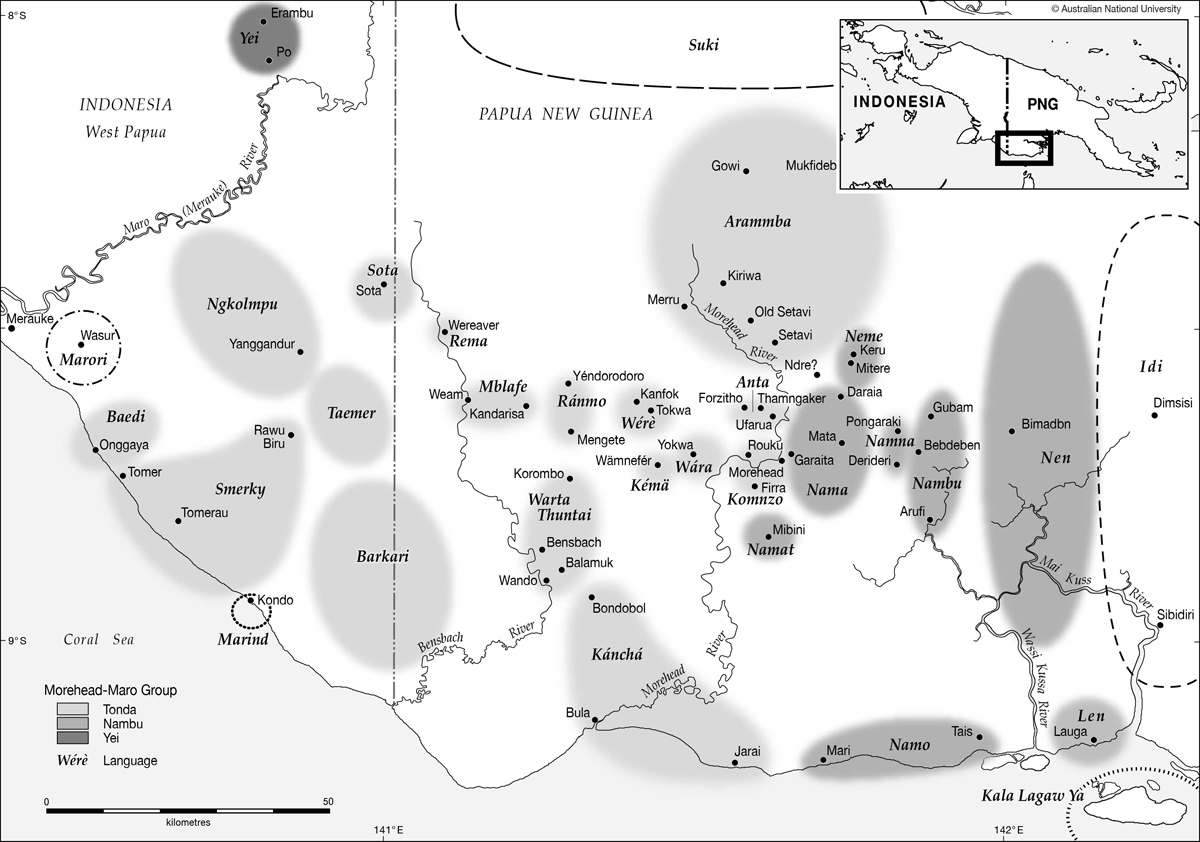
\includegraphics[width=\textwidth]{figures/map1.jpg}
	  \caption[Map of the languages of Southern New Guinea]{Map of the languages of Southern New Guinea}
	  \label{moreheadmap}
	\end{figure}
\end{landscape}

\section{Typological overview}\label{Typoverview}

\subsection{Introduction}

Komnzo is a Papuan language. The term Papuan is a negative category comprising those languages of the area near New Guinea which are neither Austronesian nor Australian. It was originally introduced by Sidney Ray (\citeyear[24]{Ray:1926papuan}). The number of distinct language families that have been proposed ranges from ten \citep{Wurm:1975etal} to 23 \citep{Ross:2005pronouns} up to 60 \citep[3]{Foley:1986ux}. Although authors acknowledge the incredible diversity within New Guinea, there have been some attempts at defining grammatical properties which are characteristic for Papuan languages (\citealt{Foley:1986ux} and \citealt{Foley:2000uh}). Komnzo, the languages of the Yam family, and possibly the whole Southern New Guinea area deviate from this Papuan type. Other authors have shown that the languages of New Guinea do not share a set of typological features that set them apart from the languages of the world \citep{Comrie:2009vza}.\\

In the following sections, I introduce the typologically most striking features of the language. Detailed information on each topic can be found in later chapters.

\subsection{Phonology}

The Komnzo phoneme inventory consists of eight vowels and 18 consonants. The vowels are the five cardinal vowels [i], [e], [a], [ɔ], [u] plus a low front unrounded vowel [æ] and, unusual for Papuan languages, two front rounded vowels [y] and [œ].\footnote{Outside of the Yam family front rounded vowels are also found in \ili{Awyu-Dumut} languages \citep[60]{vanEnk:1997tl}.} The most frequent vowel is the \isi{epenthetic vowel}, which is \isi{schwa}.

\begin{figure}[H]
\centering
	{
		\begin{vowel}[plain]
			%\caption[Komnzo vowels]{Komnzo vowels}
			\putvowel{i}{0,5\vowelhunit}{0,4\vowelvunit}
			\putvowel{y}{1,0\vowelhunit}{0,4\vowelvunit}
			\putvowel{e}{1,3\vowelhunit}{1,5\vowelvunit}
			\putvowel{œ}{1,8\vowelhunit}{1,5\vowelvunit}
			\putvowel{æ}{2,1\vowelhunit}{2,5\vowelvunit}
			\putvowel{u}{3,7\vowelhunit}{0,4\vowelvunit}
			\putvowel{a}{2,9\vowelhunit}{2,7\vowelvunit}
			\putvowel{(ə)}{2,7\vowelhunit}{1,3\vowelvunit}
			\putvowel{ɔ}{3,7\vowelhunit}{1,5\vowelvunit}
			%\putvowel{(ó)}{3,4\vowelhunit}{2,1\vowelvunit}
		\end{vowel}
	}%
	\label{vowels}
\end{figure}

The consonants follow a set of pairs of voiceless and prenasalised \isi{plosives} at the \isi{alveolar} and \isi{velar} point of articulation: [t], [\super{n}d], [k], [\super{ŋ}g]. There are labialised velars: [k\super{w}], [\super{ŋ}g\super{w}]. At the bilabial point of articulation there is only a prenasalised plosive [\super{m}b], while its oral counterpart [b] only occurs in loanwords. There are three \isi{nasals} [m], [n], [ŋ], one trill/tap [r], two semivowels [j], [w] and, again unusual for Papuan languages, three \isi{fricatives} [ɸ], [ð], [s] and two affricates [ts], [\super{n}dz]. It follows that we can identify three main points of articulation: bilabial, \isi{alveolar} and \isi{velar}. Further points of articulation are: dental [ð], palato-\isi{alveolar} [ts] and [\super{n}dz], as well as palatal [j].

\begin{table}
\label{consonants}
	\begin{tabular}{p{1cm}p{1cm}p{1cm}p{1cm}p{1cm}p{1cm}p{1cm}}
		&&t&ts&&k&k\super{w}\\
		\super{m}b&&\super{n}d&\super{n}dz&&\super{ŋ}g&\super{ŋ}g\super{w}\\
		m&&n&&&ŋ&\\
		ɸ&ð&s&&&&\\
		&&r&&&&\\
		&&&&j&&w\\
	\end{tabular}
\end{table}

Like in many Papuan languages, for example \ili{Kalam} \citep{Blevins:2010ee}, many syllables lack phonemically specified vowels. In this case, an \isi{epenthetic vowel} may be inserted, usually a short central vowel [ə]. Many words lack phonemically specified vowels altogether, like \emph{ymgthkwrmth} [jə̆mə̆\super{ŋ}gə̆θk\super{w}ə̆rə̆mə̆θ] `they were feeding him'.\\

The \isi{syllable} structure allows for complex onsets, of the type CRV as in \emph{gru} `shooting star' or \emph{srak} `boy'. Otherwise onsets are simply CV. Even though, vowel initial words exist, they are always produced with a \isi{glottal stop} as in \emph{ane} [ʔane] `that' or \emph{ebar} [ʔe\super{m}bar] `head'. Syllable codas are optional, but they consists of maximally one consonant.

\subsection{Morphology}

Komnzo morphology can be used to easily distinguish \isi{nominal}s from verbs. As in other \ili{Yam languages}, for example \ili{Nama} \citep{Siegel:2015bp} and \ili{Nen} \citep{Evans:2015to}, Komnzo \isi{verb} morphology exhibits a high degree of complexity. Verbal morphology is highly synthetic, while \isi{nominal} morphology is almost entirely suffixing.\\

Komnzo nouns are inflected for \isi{number} if their referent is \isi{animate}. Otherwise \isi{number} marking only takes place in the \isi{verb}. Furthermore, nouns are marked for \isi{case} by enclitics, which attach to the last element of the \isi{noun phrase}. Below I show the \isi{case} markers for the \isi{inanimate} noun \emph{efoth} `sun, day' and the \isi{animate} noun \emph{kabe} `man, people'.

\begin{table}[H]
\label{caseefothkabe}
	\begin{tabular}{llll}
		&inanimate&animate singular& animate non-singular\\
		Absolutive&\emph{efoth=\Zero}&\emph{kabe=\Zero}&\emph{kabe=é}\\
		Ergative&\emph{efoth=f}&\emph{kabe=f}&\emph{kabe=é}\\
		Dative&\emph{efoth=n}&\emph{kabe=n}&\emph{kabe=nm}\\
		Possessive&\emph{efoth=ane}&\emph{kabe=ane}&\emph{kabe=aneme}\\
		Instrumental&\emph{efoth=me}&\emph{kabe=me}&n/a\\
		Locative&\emph{efoth=en}&\emph{kabe=dben}&\emph{kabe=medben}\\
		Allative&\emph{efoth=fo}&\emph{kabe=dbo}&\emph{kabe=medbo}\\
		Ablative&\emph{efoth=fa}&\emph{kabe=dba}&\emph{kabe=medba}\\
		Associative&\emph{efoth=ä}&\emph{kabe=r}&\emph{kabe=ä}\\
		Characteristic&\emph{efoth=ma}&\emph{kabe=anema}&\emph{kabe=anemema}\\
		Proprietive&\emph{efoth=karä}&\emph{kabe=karä}&n/a\\
		Privative&\emph{efoth=mär}&\emph{kabe=mär}&n/a\\
		Similative&\emph{efoth=thatha}&\emph{kabe=thatha}&n/a\\
		Purposive&\emph{efoth=r}&n/a&n/a\\
	\end{tabular}
\end{table}

Nominal morphology in Komnzo is comparatively simple, with \isi{case} marking shown by enclitics which attach to the rightmost element of a noun phrase, which is usually the \isi{head} noun (\ref{exintro2}), but sometimes it may be a modifier (\ref{exintro3}).

\begin{exe}
	\ex \label{exintro}
	\begin{xlist}
		\ex
		\gll \emph{kafar} \emph{kabe=f=nzo}\\
		big man=\Erg=\Only\\
		\trans `only the big man (did sth.)'
		\label{exintro2}
		\ex
		\gll \emph{kabe} \emph{kafar=f=nzo}\\
		man big=\Erg=\Only\\
		\trans `only the big man (did sth.)'
		\label{exintro3}
	\end{xlist}

\end{exe}

In contrast to \isi{nominal}s, \isi{verb} morphology is highly synthetic. Verbs may index up to two arguments showing agreement in \isi{person}, \isi{number} and \isi{gender}. Verbs encode 18 TAM categories, \isi{valency}, \isi{directionality} and \isi{deictic} status. Complexity lies not only in the amount of categories verbs expressed, but also in the way how these are encoded.

\subsection{Distributed exponence}

Komnzo verbs exhibit what can be called ``\isi{distributed exponence}''. Distributed \isi{exponence} is characterised by the fact that morphemes are underspecified for a particular grammatical category. Therefore, morphological material from different sites has to be taken into account. This phenomenon is different from \isi{multiple exponence} (e.g. circumfixes) in that each morphological site can be manipulated independently. This is shown below in the expression of a few selected TAM categories for the verb \emph{thoraksi} `arrive, appear' in a third singular masculine frame.

\begin{table}[H]
\label{thoraksi}
	\begin{tabular}{ll}
		non-past imperfective & \emph{y-thorak-wr}\\
		recent-past imperfective & \emph{su-thorak-wr}\\
		recent-past durative & \emph{y-thorak-wr-m}\\
		recent-past perfective & \emph{sa-thor}\\
		past imperfective & \emph{y-thorak-wr-a}\\
		past durative & \emph{su-thorak-wr-m}\\
		past perfective & \emph{sa-thor-a}\\
		iterative & \emph{su-thor}
	\end{tabular}
\end{table}

Distributed \isi{exponence} means that we cannot \isi{gloss} the prefix \emph{y-} for a \isi{tense} value, because it is used for the inflections of \isi{non-past}, \isi{recent past} and \isi{past}. Furthermore, glossing the suffix \emph{-m} as a \isi{durative} is only half of its function as it backshifts \isi{tense} as well from \isi{non-past} to \isi{recent past} and again from \isi{recent past} to \isi{past} \isi{tense}. In fact, the only morpheme in the above example that serves only one function is the \isi{past} suffix \emph{-a}. As we can see in the example, exponents of TAM include the verb stem (\emph{thorak} versus \emph{thor}). Indeed, most Komnzo verbs possess two stems which are sensitive to \isi{aspect}. Again, the stem alone is not sufficient to express the aspectual values (\isi{imperfective}, \isi{perfective}, \isi{iterative}, \isi{durative}), but it is the combination of stem type, prefix and suffix.\\

Distributed \isi{exponence} is best explained with the way Komnzo marks \isi{number} on verbs. The four possible values are \isi{singular}, \isi{dual}, \isi{plural}, and \isi{large plural}. Note that only a small subset of verbs can form large plurals. The exponents of \isi{number} are distributed over two morphological slots. There is a binary distinction in the prefix (\emph{y-} vs. \emph{e-}) and the suffix (\emph{-thgr} vs. \emph{-thgn}). The four possible combinations of these exponents encode the four \isi{number} values. This is shown with the intransitive verb \emph{migsi} `hang' in a third person frame below:

\begin{table}[H]
\label{migsi}
	\begin{tabular}{ll}
		\isi{singular} & \emph{y-mi-thgr}\\
		\isi{dual} & \emph{e-mi-thgn}\\
		\isi{plural} & \emph{e-mi-thgr}\\
		\isi{large plural} & \emph{y-mi-thgn}\\
	\end{tabular}
\end{table}

\subsection{Syntax}

Komnzo is a double-marking language. The \isi{case} marking is organised in an \isi{ergative}/\isi{absolutive} system. In addition to three core cases (\isi{absolutive}, \isi{ergative} and \isi{dative}), there are 14 semantic cases. Verbs index up to two arguments. The \isi{undergoer} argument is indexed by a prefix and the actor argument is indexed by a suffix. One-place predicates split along the lines of stative versus dynamic event types. The latter employ the suffix for indexing, while the former make use of the prefix. Valency changing morphology enables the indexing of a \isi{goal}, \isi{beneficiary} or \isi{possessor} in the prefix. This is shown below with the verbs `stand', `return', `see' and `give'. I use the term ``\isi{template}'' to describe the different inflectional patterns in which verb stems are found.

\begin{exe}
\ex
\label{exintro4}
\begin{xlist}
	\ex %\textit{fi ykogr.}\\
	\gll \emph{fi} \emph{y-rugr}.\\
	\Third.\Abs{} \Tsg.\Masc-sleep\\
	\trans `He sleeps.'
	\ex %\textit{fi ŋamränzrth.}\\
	\gll \emph{fi} \emph{ŋabrigwr-th.}\\
	\Third.\Abs{} return-\Tpl\\
	\trans `They return.'
	\ex %\textit{nafa fi yfnzrth.}\\
	\gll \emph{nafa} \emph{fi} \emph{y-mar-th}.\\
	\Tpl{}.\Erg{} \Third.\Abs{} \Tsg.\Masc-see-\Tpl{}\\
	\trans `They see him.'
	\ex
	\gll \emph{nafa} \emph{yare} \emph{kabe=n} \emph{y-a-rithr-th}.\\
	\Tpl{}.\Erg{} bag(\Abs) man=\Dat{} \Tsg.\Masc-\Vc-give-\Tpl{}\\
	\trans `They give the man the bag.'
\end{xlist}
\end{exe}

The most frequent word order in Komnzo is \isi{SOV}, more accurately AUV\footnote{AUV: actor undergoer verb.}, since there is only weak evidence for a subject category. At the same time, the flagging of \isi{noun phrase}s with \isi{case} allows for considerable freedom in the word order patterns. Nominal compounds and \isi{noun phrase}s are typically \isi{head} final, although modifying elements in the \isi{noun phrase}, for example adjectives or quantifiers, may occur after the \isi{head}. Relative clauses follow their \isi{head}.\\

Subordinate clauses in Komnzo are usually non-finite employing nominalised verbs with appropriate \isi{case} markers. Verb chaining and the distinction between medial and final verb forms, which are typical for Papuan languages, are not found in Komnzo. The examples below show a phasal \isi{complement} (\ref{exintro5}) and a \isi{complement} of desire (\ref{exintro6}).

\begin{exe}
	\ex
	\gll \emph{nafa} \emph{with} \emph{rku-si} \emph{the-thkäfa-th}.\\
	\Tnsg.\Erg{} banana({\Abs}) knock.down-\Nmlz{} \Stpl-start-\Stsg\\
	\trans `They started knocking down the bananas.'
	\label{exintro5}
\end{exe}

\begin{exe}
	\ex
	\gll \emph{fi} \emph{miyo} \emph{yé} \emph{nge} \emph{fatha-si=r}.\\
	\Third.\Abs{} desirous \Tsg.\Masc.be child hold-\Nmlz=\Purp{}\\
	\trans `He wants to hold the child.'
	\label{exintro6}
\end{exe}

In addition to nominalised verbs, clauses may be connected with conjunctions (\ref{exintro7}), relative pronouns (\ref{exintro8}) or demonstratives flagged for case (\ref{exintro9}).\\

\begin{exe}
	\ex
	\gll \emph{fi} \emph{z} \emph{zebnaf}-\Zero{} \emph{o} \emph{komnzo} \emph{y-rugr}?\\
	\Third.\Abs{} \Iam{} wake.up-\Tsg{} or still \Tsg.\Masc-sleep\\
	\trans `Did he wake up already or is he still sleeping?'
	\label{exintro7}
\end{exe}

\begin{exe}
	\ex
	\gll \emph{kabe} \emph{sa-thor} \emph{kayé} \emph{mane} \emph{sf-marwrm-e}.\\
	man(\Abs) \Tsg.\Masc-arrive yesterday which \Tsg.\Masc-see-\Fpl\\
	\trans `The man who we saw yesterday arrived.'
	\label{exintro8}
\end{exe}

\begin{exe}
	\ex
	\gll \emph{ŋare} \emph{z} \emph{ze-far} \emph{bäne=ma} \emph{nafane} \emph{kkauna} \emph{zwa-rithr-th}.\\
	woman(\Abs) \Iam{} \Tsg.\F-set.off \Dem:\Med=\Char{} \Tsg.\Poss{} things \Tsg.\F-give-\Tpl\\
	\trans `The woman has left already, because they gave back her belongings to her.'
	\label{exintro9}
\end{exe}

\section{The Farem people and their language}\label{faremlang}

\subsection{Location}\label{location}

The area considered in this study is the southwestern corner of the Western Province of Papua New Guinea. This area used to be called ``Trans-Fly'' in the past, for example in Williams' ethnography of the \ili{Keraki} people entitled ``Papuans of the Trans-Fly'' (\citeyear{Williams:1936transfly}). Mary Ayres rightly criticises this term for its geo-centrism (\citeyear[1]{Ayres:ws}). I use the administrative term ``Morehead district'' which encompasses the area between the Indonesian border to the west, the Fly River to the north, the boundary of the Yam language family in the east (See Figure \ref{moreheadmap} above), and the coastline in the south.\footnote{The Morehead-Rural census division encompasses the same area, but the eastern border is further to the east including some of the \ili{Pahoturi River} languages, for example \ili{Idi}.} The area is named after Morehead station, the administrative center, and the Morehead River, which in turn was named after Boyd Dunlop Morehead, the premier of Queensland between 1888 and 1890. I use the term ``Southern New Guinea'' which encompasses a much wider region roughly from the Digul River in the west to the Fly River in the north and east.\\

Komnzo is spoken in the village of Rouku, which is located about 7km west of Morehead and about a kilometer north of the Morehead River. It is situated on the road that connects Morehead with Weam in the west. Traditional lands expand about 20km east-west and 25km north-south. There are four clans in Rouku village: \emph{Mrzar Mayawa, Banibani Mayawa, Muthrata Sangara, Wazu Sangara}.\footnote{Mary Ayres avoids using the word `clan' (\citeyear[142]{Ayres:ws}), instead she draws a distinction between ``non-local sections'' (\emph{Bagu, Mayawa, Sagara}), which are found throughout the region, and ``local-sections'' (\emph{Nümgar Bagu, Mrzar Mayawa, Muthrata Sangara}), which are found in one group only, for example the Farem. I will use `clan' for the latter and `section' for the former. This is discussed in \S\ref{exogamy}.} Further settlements include Morehead, Gunana, Firra, Kanathr, Ŋazäthe and Masu. Only Morehead and Gunana are settled permanently, while the others are garden places in some years. The map in Figure \ref{fig:map2} shows Rouku and the surrounding places.

\begin{figure}[H]
  \centering
    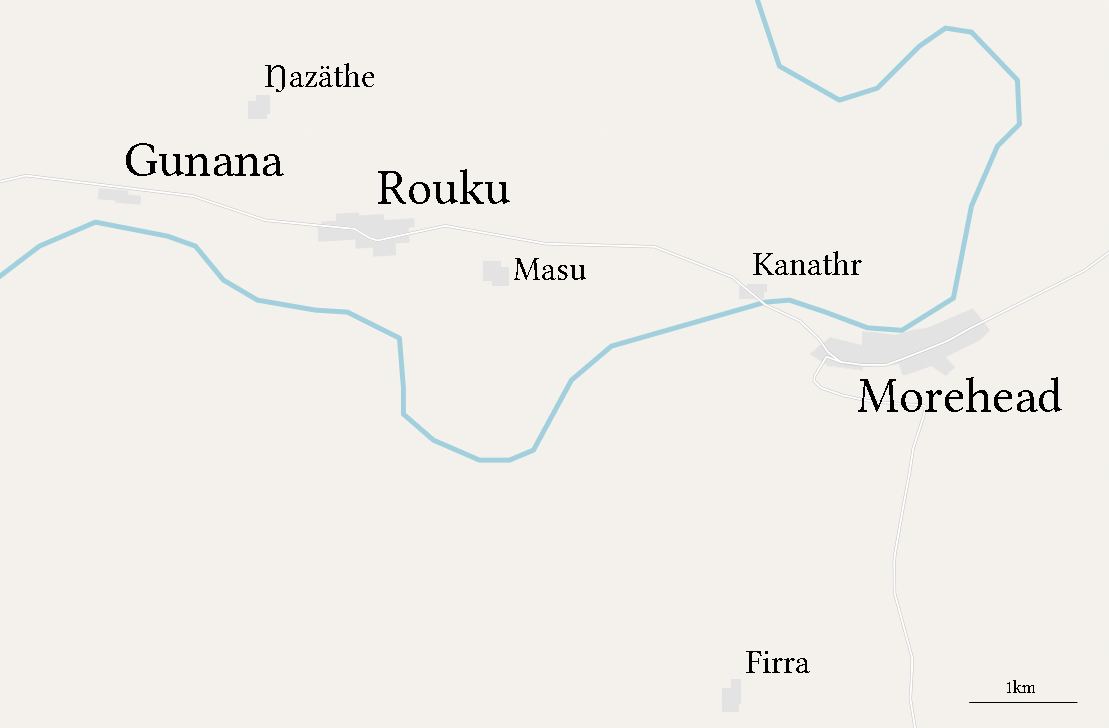
\includegraphics[width=.9\textwidth]{figures/map2.png}
  \caption[Rouku]{Rouku and surrounds}
  \label{fig:map2}
\end{figure}

Gunana, the second largest settlement, is situated about 2km west of Rouku along the road. The present-day village was established around 10 years ago. Gunana is situated closer to the Morehead River. The name Rouku, from the Komnzo word \emph{rokuroku} `riverbank', was given to this place when the first missionaries arrived in the 1950's. Thus, Gunana is the original Rouku, and it is often referred to as Rouku-Gunana. The word \emph{gunana} is a \isi{loanword} from Motu which means `old'. Two clans live at Gunana today: \emph{Farem Sangara} and \emph{Nümgar Bagu}. They speak mostly \ili{Wára} and \ili{Anta} for reasons which I address in \S{}\ref{ideomulti}. Morehead station includes the government administration, the aidpost, the primary school and the airstrip. A number of small settlements are built around Morehead station, and these virtually merge into one another. The largest of these is Garaita, a \ili{Nama} speaking village. Since Morehead station was built on land belonging to the Mayawa section from Rouku, some families from Rouku have settled in Morehead permanently. One small hamlet of this kind is Fsan. Moreover, some families from Rouku live in Morehead because they are employed in the local administration as teachers or public servants. With respect to clans, this population is mixed. The hamlet Firra is situated about 7km south of Morehead. Only a few families of the \emph{Banibani Mayawa} clan live there. Most of the people have shifted their residence to Morehead, but keep garden places at Firra. Kanathr is a small hamlet located 2km west of Morehead on the northern side of the river. Kanathr marks the point where the road crosses the river. As there is no bridge, people cross the river by canoe, and cars or motorcycles use a rusty old pontoon. Kanathr serves as a place where children from Rouku and Yokwa, the next village along the road to the west, stay overnight while they attend Morehead primary school. Kanathr was settled in the 1980's, deserted in the 90's, and re-established over the last three years. Its population is mixed with respect to clans, but since the land belongs to the two Mayawa sections, they make up the majority.\\

There are many places around Rouku which used to be settled, but have now been abandoned or are used only as garden places. These include Ytkum, Dmädr, Faremkar, Ŋazäthe, Masu and Akrimogo. Two examples are Ŋazäthe and Masu. The map in Figure \ref{fig:map2} shows Ŋazäthe, Rouku and Masu. Both used to be settled until about 10 years ago by clans of the \emph{Sagara} and \emph{Mayawa} section respectively. Today both are used as garden places, but they still play an important role as origin places. Both places are very close to Rouku, about a 15-minute walk. Note that named places are densely clustered in the Morehead district, especially in the vicinity of settlements. More importantly, places are perceived as different regardless how close they are geographically. This topic is discussed in \S\ref{placenames}.

\subsection{Geography and environment}\label{geographyenviro}

In its biota, the Morehead district is more similar to northern Australia than to the rest of New Guinea. We find eucalypts, melaleuca, acacias and banksias combined with wallabies, bandicoots, goannas, taipans and termite mounds. The area consists of lowland which a Papuan highlander or a European would describe as almost featureless. Williams describes it as having a ``mild, almost dainty, attractiveness in detail, but [...] on the whole the extreme of monotony'' (\citeyear[1]{Williams:1936transfly}).

\begin{figure}[H]
  \centering
    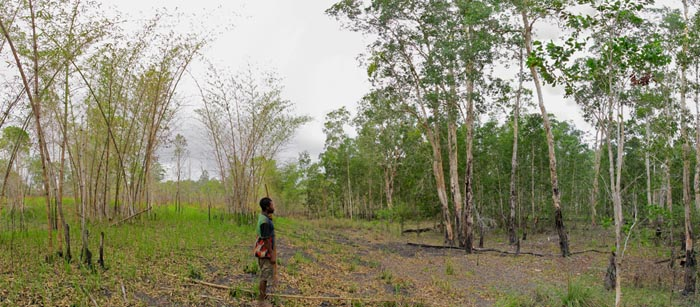
\includegraphics[width=.9\textwidth]{figures/landscape1.jpg}
  \caption[The highest water level during wet season]{Rouku: the area to the right is inundated during wet season}
  \label{fig:landscape1}
\end{figure}

I have measured differences in elevation between 12m and 41m above sea level.\footnote{This was done with a GPS device: the 12m point was the water-level of the Morehead River close to Rouku; the 41m point was measured in Rouku village.} However small these differences in elevation, they are significant over the monsoon cycle with a long dry season (June - November) and an intense wet season (January - May). Areas very close to settlements or gardens are inundated during the wet season, while the larger villages are situated on higher ground. In fact all villages along the road are built on what is called the ``Morehead ridge'' (\citealt[15]{Paijmans:1971morehead}), thus keeping houses and gardens safe from the annual flooding. The photo in Figure \ref{fig:landscape1} was taken in Rouku. During previous wet season, the paperbark trees to the right were inundated to about 1m, while the bamboo groves on the left stayed dry.\\

The Morehead ridge is intersected by many small creeks, which carry little or no water during dry season. The Morehead River always carries water as it slowly meanders towards the coast. The Morehead forms a narrow, deep channel whose riverbanks drop off sharply 2-3m down to the water level. Close to Rouku village, I have measured 40m width and 15-20m depth during dry season. The Morehead is a tidal river which means that during dry season, when it has virtually no flow, salt water pushes back many kilometers upriver. During rainy season, the river overflows and turns the surrounding land into a wide swamp with many inlets and lagoons. The image below (Fig. \ref{fig:landscape2}) shows the Morehead River during dry season.
 \vspace{-.1cm}
\begin{figure}[H]
  \centering
  %trim={0 0.9cm 0 1cm}, clip=true,
    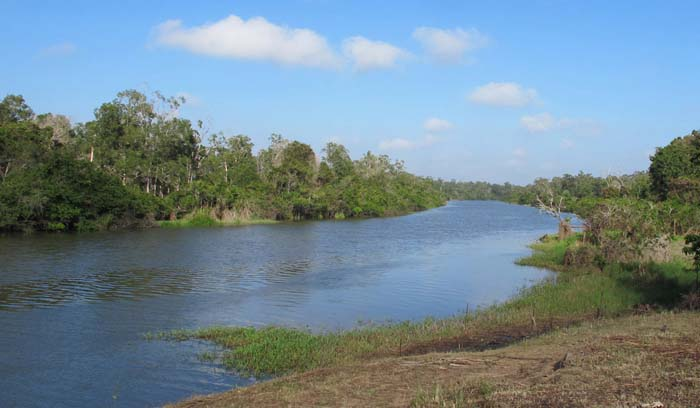
\includegraphics[trim={0 0.3cm 0 0.3cm}, clip=true, width=.9\textwidth]{figures/landscape2.jpg}
  \caption[Morehead River]{The Morehead River near Rouku during dry season}
  \label{fig:landscape2}
\end{figure}
 \vspace{-.3cm}

There is a remarkable diversity of ecological zones (\citealt{Paijmans:1970bl} and \citealt{Paijmans:1971morehead}). For the description of native land use, Ayres distinguishes four \isi{landscape} types: ``big bush'', ``open bush country'', ``clear places'', and ``seasonal swamps'' (\citeyear[5]{Ayres:ws}). In the following, I employ the respective Komnzo terms: (i) \emph{kafar fz} `big forest' is a type of monsoon rainforest, (ii) \emph{fz} `forest' is a much thinner forest type which is covered by a grass floor and dotted with red anthills, (iii) \emph{ksi kar} `bushy place' is a type of savannah which lacks trees, but is covered with high grass, and (iv) \emph{zra} `swamp' is a place entirely inundated during the wet season timbered by paperbark trees and a ground cover of dead leaves. Figures \ref{fig:landscape3}-\ref{fig:landscape6} show images of these types in the vicinity of Rouku village. As one would expect, these \isi{landscape} types differ strongly in the kinds of plants that grow there. The collection of specimens and their identification was greatly facilitated by Kipiro Damas, who visited Rouku in 2011 and 2015.\\

The Morehead district is rich in wildlife. The main game species are pigs, cassowaries and wallabies. There are many other marsupial species including bandicoots, phalangers (cuscus) and gliders. The Morehead district is also abundant in birdlife. Attested species include birds of paradise, parrots, lorekeets, pidgeons, eagles, hawks, bush fowls, jaberoos, storks and brolgas. Thanks to the help of Chris Healey, who visited Rouku in 2012 and 2013, we were able to match around 100 Komnzo bird names to the corresponding scientific names of these species. The rivers and swamps are rich in fish and amphibious species, for example barramundis, mullets, catfish, eelfish, rainbowfishes, glassfishes, stingrays, river crayfish, prawns, crocodiles, water snakes and turtles. Other reptiles include various goanna species, frogs and snakes. Examples for the latter are the Papuan taipan, the New Guinea death adder, the New Guinea brown snake, the Papuan blacksnake as well as various python types.

\begin{figure}[H]
  \centering
  	%trim={0 1.4cm 0 1.4cm}, clip=true,
    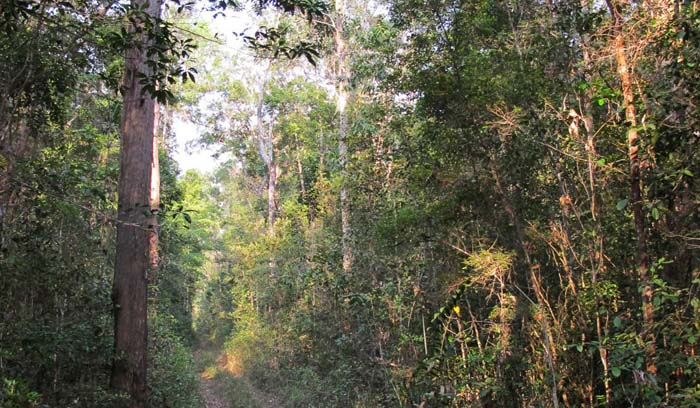
\includegraphics[trim={0 0.5cm 0 0.5cm}, clip=true, width=.9\textwidth]{figures/landscape3.jpg}
  \caption[\emph{Kafar fz}: monsoon rainforest (with a road)]{\emph{Kafar fz}: road cut through the monsoon rainforest}
  \label{fig:landscape3}
\end{figure}
 \vspace{-.6cm}
\begin{figure}[H]
  \centering
  	%trim={0 0.4cm 0 0.4cm}, clip=true,
    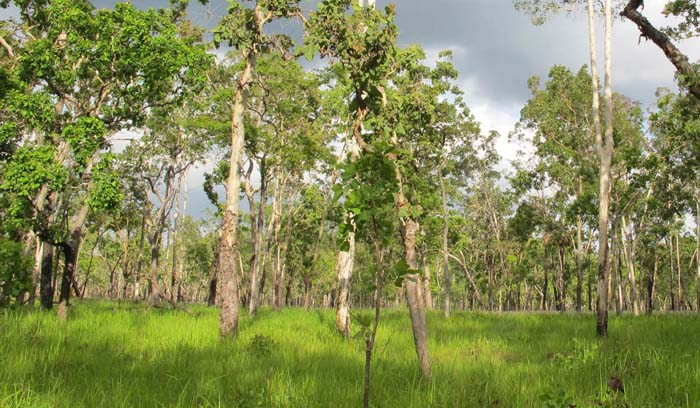
\includegraphics[trim={0 0.3cm 0 0.3cm}, clip=true, width=.9\textwidth]{figures/landscape4.jpg}
  \caption[\emph{Fz}: thin forest]{\emph{Fz}: thin forest}
  \label{fig:landscape4}
\end{figure}

\begin{figure}[H]
  \centering
    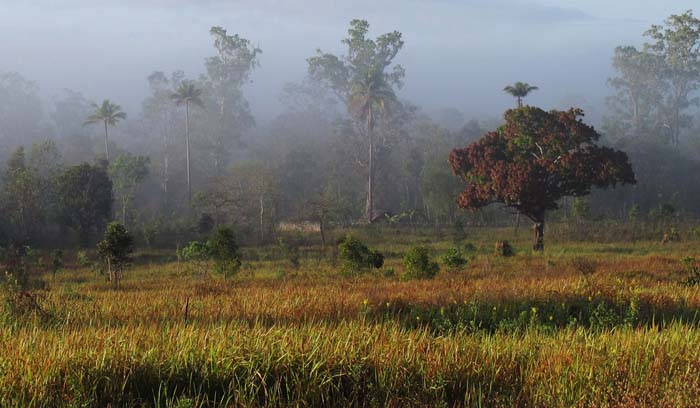
\includegraphics[width=.9\textwidth]{figures/landscape5.jpg}
  \caption[\emph{Ksi kar}: small patch of savannah]{\emph{Ksi kar}: small patch of savannah}
  \label{fig:landscape5}
\end{figure}

\begin{figure}[H]
  \centering
    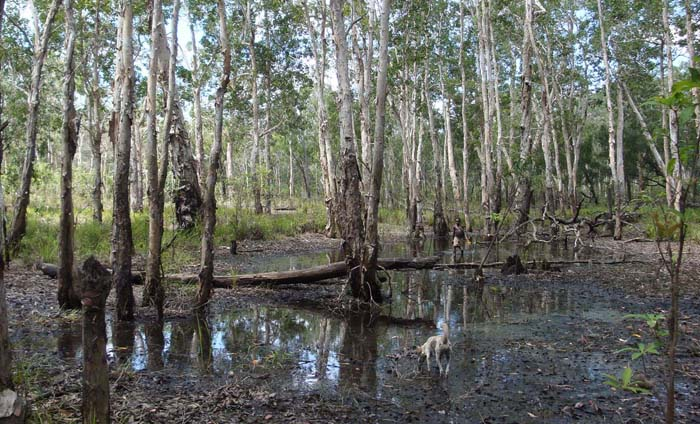
\includegraphics[width=.9\textwidth]{figures/landscape6.jpg}
  \caption[\emph{Zra}: seasonal swamp during dry season]{\emph{Zra}: seasonal swamp during dry season}
  \label{fig:landscape6}
\end{figure}

\subsection{Agriculture and subsistence}\label{agriculture}

The Farem people are agriculturalists. Their main crops are round and long yams, bananas, sweet potatoes, cassava, taro, coconut, sago, breadfruit and sugar cane. Additionally, there are many fruits and nuts available during the dry season. Although the Farem are skilled in hunting, trapping and fishing, they rely on their garden products. In this section, I focus on their staple food, which is yam.

\begin{figure}[H]
  \centering
    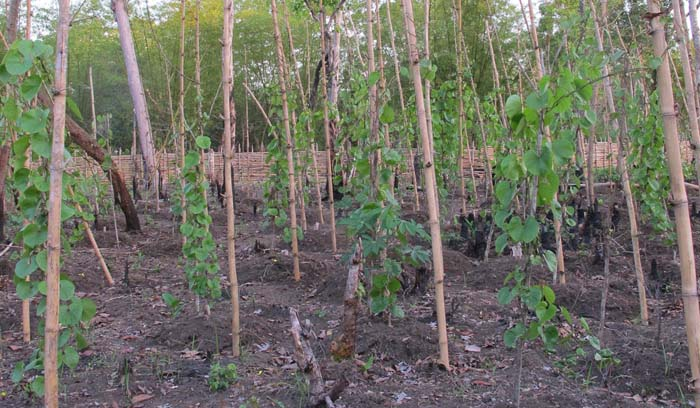
\includegraphics[width=.9\textwidth]{figures/yam1.jpg}
  \caption[Yam garden two months after planting]{Yam garden two months after planting}
  \label{fig:yam1}
\end{figure}

Without doubt yams are the most important crop for the Farem, and the role of this bland tasting tuber can hardly be overstated. FE Williams concludes his chapter on food production by stating that ``the social significance of food among these people derives largely from the pride which individuals and groups feel in having plenty of it.'' (\citeyear[235]{Williams:1936transfly}). Large quantities of yams are exchanged at feasts, and sizeable tubers are often given as personal gifts. During the celebration of Independence Day in Morehead, there is a competition where individuals measure and weigh their biggest yams. On many occasions, people have shown off the content of their yam houses to me, and during harvest time some of my friends have peeked through the wall of someone's yam house to examine the yield and compare it to their own, which often became the talk of the day. In short, yams indicate a person's wealth and social status.\\

Yam cultivation involves hard labour. The cultivation cycle can be divided into three phases: (i) preparing and planting, (ii) tending, and (iii) harvesting. The preparations begin by clearing the land (between August and October). Good, well-drained soil is found on the high ground; either virgin forest or a piece of land that has lain fallow for some years. The gardener has to cut the overgrowth and clear the grass. Large trees are usually only ring-barked and one would wait for the tree to die and eventually to fall. The cleared area has to be burned. Depending on the quality of the soil, one may bring grass from elsewhere and burn it as fertiliser. The ground has to be ploughed thoroughly, and small roots and weeds are pulled out. Next, the garden plot has to be enclosed by a fence to keep out wallabies, deer and wild pigs. The most important material for fences is bamboo which is grown in small bamboo groves. During preparation, people are busy in their gardens every day. Planting may start as early as October, but it can last until January. Yams for planting are selected carefully, but the tiny yam suckers are usually planted in heaps in an old garden plot. Figure \ref{fig:yam1} shows a yam garden about two months after planting. Between January and June, there are many small jobs to be done. These include weeding or erecting and replacing yamsticks on which the vines climb up. The change of the season in June is also signalled by the changing colour of the yam leaves. Around this time, the harvest season begins, and it may stretch until August, when the cycle begins again. Harvested yams are counted, sorted and stored in yam houses. This involves shaving the shoots off each tuber; a time-consuming task that is usually done in the afternoon hours while sitting in conversation in front of the yam house. Because garden plots are subdivided into rows, one for each member of the family, the yams are sorted accordingly in the yam house. Figure \ref{fig:yam2} shows the inside of a yam house after the harvest.

\begin{figure}[H]
  \centering
    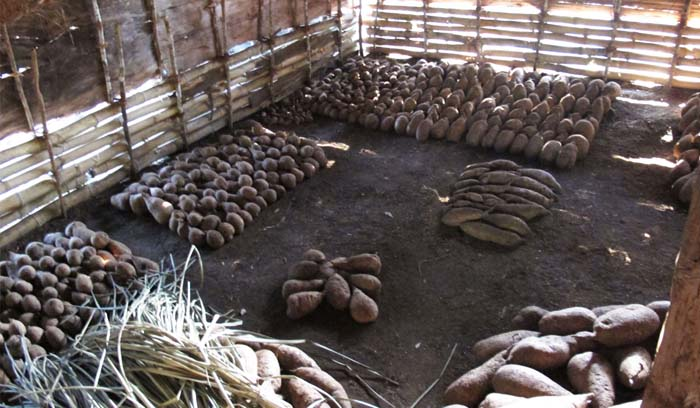
\includegraphics[width=.9\textwidth]{figures/yam2.jpg}
  \caption[Inside a yamhouse]{Inside a yamhouse}
  \label{fig:yam2}
\end{figure}

There are many special customs around yam cultivation. Some men possess yam planting magic which helps them to compete with others. This usually involves particular spells and magic stones passed down from the father's generation. Others ``steal the soil'' from their competitors. Knowledge of this kind is usually kept secret and never admitted in public. Furthermore, there are a number of rules about handling yams, which everyone follows. One example is the belief in ``female pollution'', which is widespread in Southern New Guinea (\citealt[104]{Knauft:1993south}). During a woman's monthly period, but also after having sexual intercourse, it is strictly forbidden to go to the garden plot for it will ``spoil'' the yams. This rule applies not only to the woman, but to anyone who sleeps in the same house, sometimes even the neighbouring house.\\

Yams play the most important role in exchange feasts. For example, an exchange marriage is consummated through a feast, sometimes called ``pig dance''. The two men who have exchanged sisters henceforth \emph{fäms} `exchange fellow', will raise a pig and invite their respective \emph{fäms} and his associates for a dance. The host side will feed the guests, and in return the guests will entertain the hosts by singing and dancing through the night. The next day, the hosts will give the guests large quantities of yam tubers to take back to their village. The amount has to be recorded with great detail, because after a year has passed, the roles will be reversed. Nothing would be more embarrassing than falling short in the repayment. Often two villages have particularly strong marriage links. in the past this has led to competitive yam cultivation between those two groups.\\

Yams also play a role in the regulation of conduct. I have been told about a ritual called \emph{mefa}. The culprit, usually someone who has treated his wife badly, is confronted by his \emph{fäms} and other brothers of his wife (\emph{ngom}). These will put lime on the culprit's forehead and then strike him over the head with a small yam tuber. This is, however painful, only an immediate punishment. The bigger punishment comes in the form of a gift. The culprit is given a large quantity of yams, and it is expected that he repays the same amount and quality the next year. An individual can never achieve this, and thus the culprit is forced to ask people in and maybe even beyond his clan for help. If he fails to repay the expected amount, he will lose all respect and social status. Disputes about an individual's gardening abilities may become violent. The only time I had to witness a violent outbreak by one of my brothers, who is a calm and peaceful person, was when his aunt insulted him by accusing him of ``being lazy'' and a ``bad gardener''. After a tirade of insults, this was the last straw. In conclusion, it is difficult to find any aspect of life in which yam cultivation does not play some role.

\subsubsection{Yam counting}\label{yamcounting}

For many of the customs described above, it is important to record the exact quantity of tubers. For the counting ritual a special base-six \isi{numeral system} is used, which is unique to the \ili{Yam languages}. This \isi{senary} system has received some attention in the literature (\citealt{Donohue:2008bn}, \citealt{Hammarstrom:2009bp} and \citealt{Evans:2009wg}). Williams was the first to describe the counting procedure, but he points out that it ``is apparently a more or less recent fashion among the \ili{Keraki}, having been imported from beyond the Morehead'' (\citeyear[225]{Williams:1936transfly}). This area includes the Farem territory. In the following section, I describe the procedure as I have witnessed it many times in Rouku and surrounds.\footnote{I have published two videos of the counting procedure. The interested reader can view them at the following URLs: \fbox{\href{https://vimeo.com/54887315}{https://vimeo.com/54887315}} and \fbox{\href{https://vimeo.com/21058525}{https://vimeo.com/21058525}}}\\

\begin{figure}[H]
  \centering
    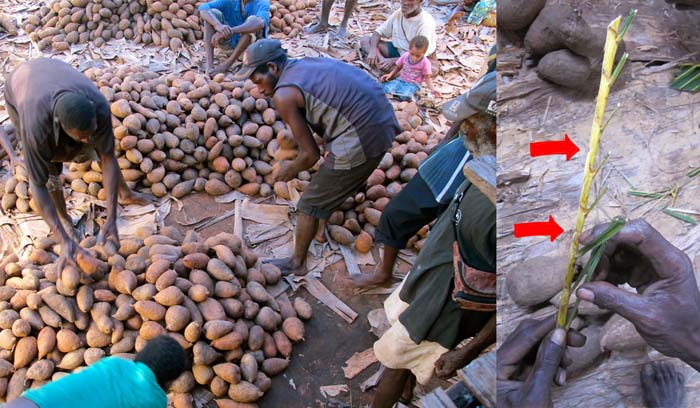
\includegraphics[width=.9\textwidth]{figures/yam3.jpg}
  \caption[Ritual yam counting]{Ritual yam counting (left); counting tally \emph{tiftif} (right)}
  \label{fig:yam3.jpg}
\end{figure}

The counting procedure involves two men who move the yam tubers from a prepared pile. They take up three yams each, move a few meters and deposit them together in a new pile. One of the two is the designated counter and he shouts out \emph{näbi näbi näbi} `one one one'. This means that they have moved the first unit of six. Without pause they take up again three yams each and move them over, while the counter shouts out \emph{yda yda yda} `two two two'. Now two lots of six or 12 tubers have been counted. Again they pick up three yams each shouting \emph{ytho ytho ytho} `three three three'. The two men continue with this process until they reach \emph{nibo} `six'. Now 36 yams have been counted and the bystanders and observers cheer up in agreement. This amount corresponds to one \emph{fta} or 6\textsuperscript{2}. Each \emph{fta} is marked by putting a single yam on the side of the new pile. The two men continue until all yams have been counted, and the little pile on the side which indicates the amount of \emph{fta} slowly grows. Next, this pile is counted in the same fashion, only that each counting yam, that is put to the side, now markes one \emph{taruba}, which corresponds to 216 or 6\textsuperscript{3}. One may continue in the same fashion. Six \emph{taruba} make up one \emph{damno} corresponding to 1,296 or 6\textsuperscript{4}. For example, one \emph{damno} is amount of yams that a man should store in order to bring his family through the year. Six \emph{damno} make up one \emph{wärämäkä} corresponding to 7,776 or 6\textsuperscript{5}. Finally, six \emph{wärämäkä} make up one \emph{wi} corresponding to 44,656 or 6\textsuperscript{6}. I should add that nobody in Rouku remembered the last time this number was actually reached. The recursive counting procedure gives rise to the \isi{senary} system. I describe the \isi{numeral system} in \S\ref{numerals}.\\

Figure \ref{fig:yam3.jpg} shows two men during the counting the procedure. The counting is always a public event accompanied by the loud, monotonous beat of the drum. I was told that neighbouring villages or travellers should be made aware of the ongoing counting procedure. In order to record and keep the amount for later proof, the Farem produce a counting tally made from a coconut frond. This is shown on the right side of Figure \ref{fig:yam3.jpg}. The stalks indicate the amount of different \isi{senary} values, which are separated by small notches. The red arrows in the image point to the two notches. Figure  \ref{fig:yam3.jpg} was taken during a yam counting ritual in Morehead in September 2010. The amount counted was 3 \emph{damno}, 2 \emph{taruba}, 3 \emph{fta} or 4,428 tubers in total. This was the contribution of several clans to a pig dance that took place two weeks later in Garaita. The counting had to be repeated two times because older men who observed the procedure closely said that mistakes had been made.\\

The largest amount of yams that I have seen was in the village of Yokwa in September 2013. Following the death of an older men, the relatives decided to built a \emph{sirä mnz}, a communal yamhouse.\footnote{Mary Ayres uses the word \emph{kwitenz} for this, but my informants from Rouku and Yokwa did not know the word. They suggested \emph{sirä mnz} `\emph{sirä} house'. The word \emph{sirä} refers to the shelves that are found in these yam houses to hold especially large tubers.} All the relatives of the deceased man, including my brother from Rouku, stored several \emph{fta} up to one \emph{taruba} of yams inside this house. The content was to be shared and exchanged during a feast in honour of the deceased at the height of the rainy season. Mary Ayres describes this practice in her chapter on mourning customs (\citeyear[289]{Ayres:ws}). The yamhouse in Yokwa can be seen in Figure \ref{fig:yam4} below. It measured 2,50m width, 1,60m height and an incredible 60m length. The floor was separated into compartments of equal size where each contributor stored his share. For some of the contributors there was a display shelf (\emph{sirä}) for very large yams. I did not witness the whole counting procedure as it took more than a day, but I estimate that the \emph{sirä mnz} held more than 10,000 yams.

\begin{figure}[H]
  \centering
    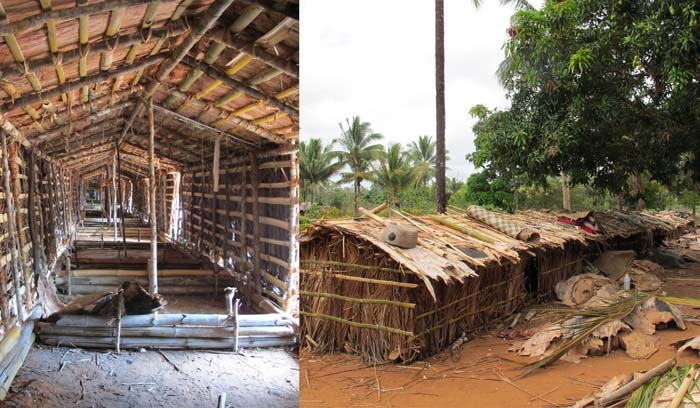
\includegraphics[width=.9\textwidth]{figures/yam4.jpg}
  \caption[Communal yamhouse in Yokwa]{Communal yamhouse in Yokwa: inside (left) / outside (right)}
  \label{fig:yam4}
\end{figure}

\subsection{Demography and vitality}

It proves difficult to determine the exact number of Komnzo speakers. I give a rough estimate here between 150 and 250. For the most part, this inexactness is caused by particular social factors. For example, the system of exchange marriage fosters a high degree of \isi{multilingualism}. A Farem child typically grows up speaking at least the varieties of her father and mother. Since the system of residence is virilocal only the father's language is Komnzo. Of course there are two sides to this, and there are many speakers of Komnzo in other villages, namely women who have married out and their children. What complicates matters further in the case of Rouku is that not all Farem men speak Komnzo as their daily language, and not all families have a Komnzo speaking parent. I provide an explanation for this in \S{}\ref{modernhistory}. Furthermore, there is a small group of speakers who have moved further away to Daru, Kiunga, Port Moresby or other parts of Papua New Guinea.\\

Komnzo is vital in the sense that the language is being transmitted to children. At the same time, Komnzo is an endangered language because of its small number of speakers and its relatively low prestige compared to the lingua franca, which is \ili{English}. Komnzo is not taught in the school system, there is no writing tradition, and it is not used at the administrational level. For these reasons, it should be regarded as an endangered language from an academic point of view.\\

Komnzo speakers perceive their language to be under threat from what they call ``mother's language''. Mary Ayres notes that there are strong marriage links between particular villages because it is desirable for a daughter to marry back to her mother's village (\citeyear[226]{Ayres:ws}). In the case of Rouku, there are strong links to Yokwa, and what is meant by ``mother's language'' is almost always \ili{Wára}. One line of reasoning about the perceived threat is that women from Yokwa fail to pass Komnzo on to their children. Note that women are expected to shift speech variety as they shift location to their husband's village. In reality this hardly ever occurs, because there are enough women from Yokwa to form small exclaves of \ili{Wára} speakers. Moreover, all Komnzo speakers are fluent in \ili{Wára}. Hence, there is little pressure on a woman to actually shift her speech variety. This is different with women who come from more distant places. I discuss the topic of \isi{multilingualism} and \isi{language ideology} in \S{}\ref{ideomulti}.

\subsection{History}\label{history}

\subsubsection{Pre-contact history}\label{prehistory}

Until the rise of the sea level during the Late Pleistocene, the island of New Guinea and the Australian continent were joined in a single landmass called Sahul (\citealt{White:1982prehist}). Recent studies have highlighted that there is still a lack of research from the Southern New Guinea region (\citealt{Pawley:2005ue}, \citealt{Ballard:2010cd}, and \citealt{Evans:2012wp}). The geomorphological past of this lowland region has been turbulent over the last 20,000 years. A chronology of the changing coastlines is given by Chappell (\citeyear{Chappell:2005coastal}).\footnote{His methodology is as follows: ``the procedure for reconstructing the coastlines at a given epoch is to compute the relative sea level field for a given region [...] by combining the ice-equivalent sea level with the regional departures that arise from the isostatic and gravitational factors. The results are then superimposed on the present topography in detail...'' (\citeyear[529]{Chappell:2005coastal}).} Figure \ref{fig:figures_chappell21k} shows the northern coastline of Sahul at the Last Glacial Maximum at 21,000 BP. Figure \ref{fig:figures_chappell8k} shows the coastline at 8,000 BP shortly after the sea breached the Torres Strait, thus disconnecting New Guinea and Australia. The thin black line shows the present coastline.

\begin{figure}[H]
  \centering
    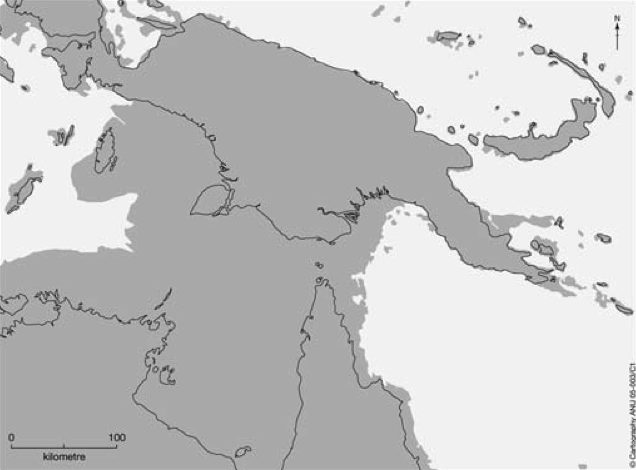
\includegraphics[width=.6\textwidth]{figures/chappell21k.png}
  \caption[Coastline at 21,000 BP]{Coastline at 21,000 BP; adopted from (\citealt[527]{Chappell:2005coastal})}
  \label{fig:figures_chappell21k}
\end{figure}

\begin{figure}[H]
  \centering
    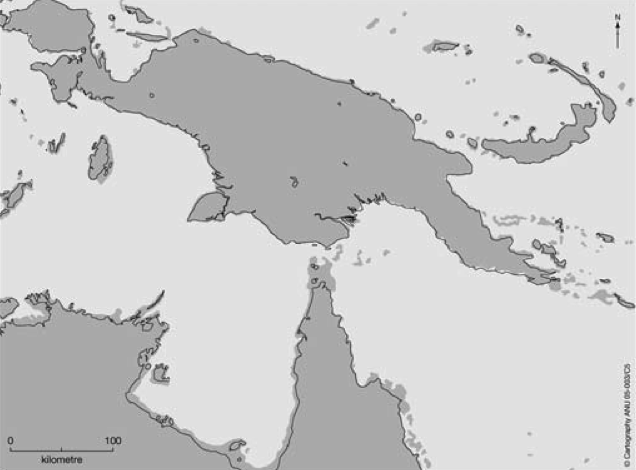
\includegraphics[width=.6\textwidth]{figures/chappell8k.png}
  \caption[Coastline at 8,000 BP]{Coastline at 8,000 BP; adopted from (\citealt[528]{Chappell:2005coastal})}
  \label{fig:figures_chappell8k}
\end{figure}

We can see from the figures that the separation of Sahul occurred only shortly before 8,000 BP. Keeping in mind that human presence on the Sahul continent goes back to at least 40,000 BP (\citealt{Golson:2005intro}), we can safely assume that what was later to become the Southern New Guinea region was already settled well before the separation. Chappell shows that large parts of the Fly-Digul platform, to which the Morehead ridge belongs, was submerged at the maximum height of the sea level at 6,000 BP. Figure \ref{fig:figures_chappell6k} shows that this has affected the western part of the Southern New Guinea region.\footnote{With regard to Figure \ref{fig:figures_chappell6k}, which is the result of a computer model, Chappell argues for a more conservative estimate, in which the coastline at 6,000 BP does not extend all the way up to the Fly River (\citeyear[531]{Chappell:2005coastal}).} This part of the region was slowly rebuilt by the sediments carried by the Fly River and Digul River. Note that the Morehead ridge as one of the highest points of elevation on the Fly-Digul platform was not submerged during this period.

\begin{figure}[H]
  \centering
    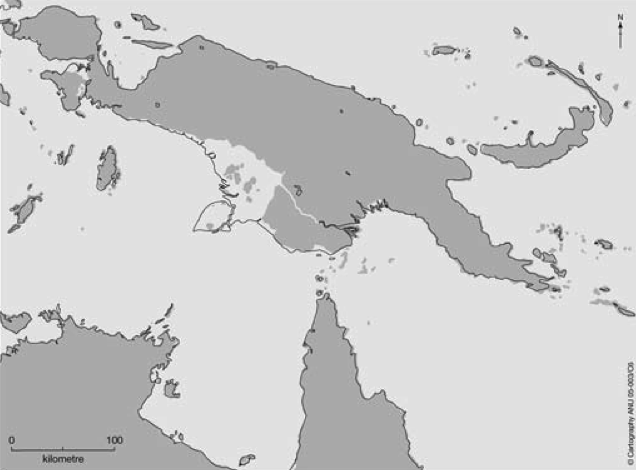
\includegraphics[width=.6\textwidth]{figures/chappell6k.png}
  \caption[Coastline at 6,000 BP]{Coastline at 6,000 BP; adopted from (\citealt[528]{Chappell:2005coastal})}
  \label{fig:figures_chappell6k}
\end{figure}

The geological scenario outlined by Chappell is reflected to some extent in the linguistic landscape of the region. For example, concerning the Trans-New-Guinea languages spoken in west of the Fly-Digul platform, Pawley points out that the ``homogeneity of the Asmat-Kamoro group is clear evidence that their expansion was comparatively recent'' (\citeyear[10]{Pawley:2005intro}). Usher and Suter (\citeyear{Usher:2015kr}) have recently shown evidence for the existence of the Anim language family which stretches from Ipiko in the east to \ili{Marind} and Yaqayic in the west, thus encircling the area concerned with in this study. Evans argues that it is ``unlikely that all language differences currently found in Southern New Guinea developed in situ. What seems more likely is that they represent the interaction of a number of unrelated groups entering the region from different regions'' (\citeyear[111]{Evans:2012wp}). While this is evident for some of the linguistic units, for example the Trans-New-Guinea languages, we do not know how other linguistic units, for example the \ili{Yam languages} or the \ili{Pahoturi River} languages, fit into the chronology of events. I suggest that we should accept the possibility that the \ili{Yam languages} represent a much older population, and {\textendash} as Evans rightly point outs {\textendash} we can only speculate from where this population has entered the region.\\

Some suggestions come from recorded mythology, namely the myth of two brothers and the origin of people at a place called \emph{Kwafar}. This myth was recorded by FE Williams (\citeyear[306]{Williams:1936transfly}) as well as Mary Ayres (\citeyear[50]{Ayres:ws}). I have recorded a version of this myth told in Komnzo, which is given in the Appendix \ref{kwafar}. What is noteworthy about the story is that the place \emph{Kwafar} is located off the coast in an area that was last exposed well before 8,000 BP. Events told in the story led to a flood and the  ancestor escaped northwards. Eventually, he picked up the branches of \emph{dödö} `Melaleuca sp', beat the water with it, and the flood came to a halt. The myth suggests that the people have retreated northwards from the rising sea level, i.e. the myth ``reports'' events which date back at least 8,000 years. Although I am not claiming linguistic continuity from the time of the sea level rise to present-day Komnzo {\textendash} after all we know that populations may shift languages {\textendash} one cannot deny the fact that this myth is found in the area where the \ili{Yam languages} are spoken, more precisely the languages of the \ili{Tonda} subgroup.\footnote{Both Williams and Ayres have recorded these myths with speakers of Tonda languages. Among the origin myths of the Morehead district, this particular myth is only found in Tonda speaking territory.}

\subsubsection{Modern history}\label{modernhistory}

The Southern New Guinea region was contacted relatively late, which led Knauft to claim that it has ``remained effectively outside the purview of state political economies for longer than any other major non-arctic coastal population'' (\citeyear[26]{Knauft:1993south}). In 1890, Sir William MacGregor, the Administrator of Papua, discovered the Morehead River on an expedition. It took another six years for a second visit by MacGregor during which he collected a vocabulary list, which can be found in the Annual Reports (\citealt[106]{MacGregor:1896rep}).\footnote{Based on the verb forms in the list, I identify the variety as either \ili{Kánchá} or \ili{Kémä}. Nominalised verbs in these two varieties end in a bilabial fricative, and many verbs in the list have a final grapheme <p>. In Komnzo, \ili{Wára}, \ili{Anta} and \ili{Wèré} nominalised verbs end in a vowel: [i] or [e].} Both expeditions travelled by ship. The first known white man to walk through the region was William Dammköhler in 1898 on an adventurous escape from \ili{Marind} headhunters (\citealt{Hitchcock:2009gg}). Until 1921, sporadic patrols were conducted by AP Lyons, Resident Magistrate of the Western Division. Lyons recorded native customs, but his journals held at the National Cultural Council at Port Moresby were inaccessible to me. In 1926, FE Williams started to pay regular visits to the Morehead district in his role as ``official government anthropologist''. Until 1932, he visited the area almost every year, and his fieldwork culminated in the book Papuans of the Trans-Fly (\citealt{Williams:1936transfly}), which is still the most comprehensive ethnographic description of a group in the Morehead district.\\

At the time of contact, Southern New Guinea was home to groups of very different sizes and political organisation. On the one end of the spectrum, there were small groups like the Farem, probably with no more than 100 people at that time. On the other end, we find large groups like the \ili{Kiwai} (9,700), \ili{Marind} (7,000) and \ili{Suki} (3,500). Note that these three groups surround the area concerned with in this study. Although headhunting was practised by all groups, it was only those larger groups which could muster war parties and attack places far away from their home territory. This was especially true of the \ili{Marind} (also known as Tugeri or Tugere). In his introduction to Williams' book, AC Haddon, who had led the British expedition in the Torres Strait in 1888, writes that he had ``heard lurid stories about these head-hunting, cannibal marauders'' (\citeyear[xxiiv]{Williams:1936transfly}). The \ili{Marind} were militaristic expansionists, who went on headhunting expeditions raiding villages along the south coast as far as Boigu Island. Since the \ili{Marind}'s home territory was in Dutch New Guinea, the British colonial administration was unable to act against them. The \ili{Marind}'s activity led to a joint Dutch-British expedition, which established the border at the mouth of the Bensbach River. Eventually, in 1902, the Dutch administration set up a police post in Merauke.\\

The impact of the \ili{Marind} is somewhat inconclusive. For example, Mary Ayres argues that their immediate role has been overstated by many Europeans who have visited the area in this early period (\citeyear[19]{Ayres:ws}). She points to two confusing inferences that had been made. The first was the erroneous belief that a great number of settlement names given to MacGregor and various patrol officiers must also mean that the population of the Morehead district must be very large. As I explain below, the traditional settlement pattern was to live in small hamlets often comprising a single patriline. Secondly, the fact that the population density was actually very low was attributed to massive depopulation by the \ili{Marind}. An example comes from MacGregor who describes that he met a group of people on the Morehead River: ``Of this tribe we saw altogether about thirty to forty men, boys and women. They are probably the remains of a tribe that has been decimated by the Tugere'' (\citeyear[74]{MacGregor:1890rep}). Ayres criticises that MacGregor and others jump to conclusions here. The low population density in the Morehead district, especially along the coast west of the Wassi Kussa River, can be explained by geographical factors alone. She notes that ``the accute scarcity of fresh water during the dry season was not readily observed'' (\citeyear[22]{Ayres:ws}), because early visits always occurred during the rainy season, which is the best time to navigate the coast. Ayres concludes that there is no definite evidence for or against depopulation by the \ili{Marind}. Nonetheless, if we consider the discrepancies in group sizes in Southern New Guinea over a longer period, it is easy to imagine that these larger groups would have assimilated the smaller ones sooner or later. Evans concludes that ``we may not be exaggerating to say that without the arrival of colonial governments (and missionary endeavours eliminating headhunting and overt warfare) many of the small languages of the Trans-Fly may not have survived in the way they have.'' (\citeyear[117]{Evans:2012wp}).\\

In the remainder of this section, I will focus more on the local level. In 1951, the administration established a government station at Rouku. The name Rouku comes from Komnzo \emph{rokuroku} `riverbank'. This name was given to a place a few kilometers to the west of present-day Rouku, where a group of Farem people had lived in the 1920's (\citealt[14]{Ayres:ws}). This older Rouku is now settled again by Farem people who call it Gunana {\textendash} a Motu word meaning `old' {\textendash} and sometimes it is called Rouku Gunana `old Rouku'. The government station included a school, which was run by the London Missionary Society. Its successor, the United Church, is still the most influential denomination in the area west of Morehead, including Rouku. During the 1950's, the Australian Petroleum Company explored the Morehead district for oil. Many older Farem still remember their parents being employed as labourers with the company. A more tangible legacy of the company's operation is a network of roads in the Morehead district, although these have often reverted back to narrow tracks. In 1959, the station was shifted to Morehead, where an airstrip was constructed. In the early 1960's, a government school was opened there, which has been operational until today. Since that time, Morehead has been the administrational centre of the district.\\

Large bureaucracies like nation-states tend to organise their population by dividing and subdividing them into organisational units. The nation-state Papua New Guinea consists of 22 provinces, which consist of districts, which in turn consist of local level government areas, which are divided into wards. Rouku belongs to Ward 16 of the Morehead-Rural local level government area of the South Fly District of Western Province. Such organisational schemes are useful, but they fail to adapt to cultural peculiarities, an issue which seems of particular importance in a country as diverse as Papua New Guinea. During the 1950's and 1960's, the government began a policy of village consolidation. Small hamlets and related villages were asked to form combined larger villages. The concurrent establishment of churches, schools and roads provided some incentives for this policy to show some effect. I agree with Ayres when she writes that this ``is antithetical to traditional settlement patterns of widely scattered very small villages where residence is not continuous'' (\citeyear[17]{Ayres:ws}). It is no surprise that people returned to their traditional settlement patterns during the 1970's when the government patrols ceased. Thus, on a very local level we find a pulsating movement from dispersion to consolidation and back to dispersion. Ayres supports this observation by pointing out that {\textendash} although Rouku was consolidated as `one village' during the 1950's {\textendash} the Farem people lived scattered over several hamlets when she did fieldwork in 1980. The official census for Rouku in 1980 was 108, but only 30 people lived at Rouku then (\citeyear[17]{Ayres:ws}). The others lived at Ŋazäthe, Faremkar, Kafthéfr, Masu, Firra, Kanathr and Morehead.\\

30 years later, I can add my own observations to this. When I first visited Rouku in 2010, my main informant Abia Bai told me that he had lived in Kanathr in the 80's and later at Masu together with his Mayawa clan (\emph{Mrzar Mayawa}). In the mid-1990's, this clan moved from Masu to Rouku, thus Masu and Kanathr were not settled in 2010. Two Sagara clans (\emph{Muthrata Sagara} and \emph{Wazu Sagara}) had lived in Rouku more or less continuously with short intervals at Ŋazäthe and Faremkar. In 2010, the Bagu clan (\emph{Nümgar Bagu}) was transitioning to Gunana from a place called Dmädr, about 5km to northwest of Rouku. Gunana itself was established around the year 2000 by the third Sagara clan (\emph{Farem Sagara}). Lastly, the second Mayawa clan (\emph{Banibani Mayawa}) was split between one patriline living in Rouku and another patriline living in Morehead. The latter had moved to Morehead from Firra during the late 1990's. Hence, we could say that in 2010 the Farem people were ``consolidated'' in the two settlements of Rouku and Gunana. Over the last five years, some of the Mayawa people have established a new settlement at Kanathr. What started out with two families in 2012, has now grown to about four families which belong to both Mayawa and Sagara. Other people have built houses in Masu and Ŋazäthe. Yet others have moved to Morehead. The point I am trying to make is that settlement is not continuous and an individual may choose to move several times during his lifetime. During the annual cycle, movement is even more pronounced as one may stay for several weeks at a garden place during the planting and harvesting time, or at a sago, fishing or hunting camp. As a consequence, I have often arrived in Rouku wondering where all the people had gone.\\

An interesting epiphenomenon to oscillation between fragmentation and consolidation is that it did not always follow linguistic or cultural lines. For example, the closest village to Rouku is Yokwa (also called Safs) situated about 12km west along the road. During the first consolidation in the 1950's, people from the south who spoke \ili{Kánchá} and Ara consolidated with the \ili{Wára} speakers of Yokwa. Naturally, this may lead to problems in the documentation of a particular speech variety. While it is easy to find \ili{Kánchá} speakers for comparison further to the south in other villages, \ili{Wára} and Ara speakers are only found in Yokwa. I should add that I have not had the opportunity to study this in detail in Yokwa.\\

For the linguistic history of Rouku, this meant that some men of the father generation of the Bagu clan as well as two of the Sagara clans had shifted to Yokwa and lived there for almost a decade. Nowadays, their children live in Rouku and Gunana, and despite being bilingual in Komnzo and \ili{Wára} they speak mostly \ili{Wára}. This is not only a problem for the documenter, but it results in real political problems. As I point out in \S{}\ref{ideomulti}, the linguistic ideology in the Morehead district connects identity with land and language. Consequently, there is a strong feeling that one should speak the variety that in some sense belongs to the land. In other words, a Farem individual should speak Komnzo. It follows that for some individuals village consolidation has led to a disconnect between the daily language and the language of social identity.

\subsection{Mythology and the origin of people}\label{mythology}

Ayres (\citeyear[146]{Ayres:ws}) uses the term ``starting-place'' to describe the place from which the apical ancestor of each group has spread. I will label these ``origin places'' henceforth. There are multiple origin places because there were multiple splitting events. The notion of spreading from a prior unity is pervasive in the Morehead district, and Ayres offers a spatial analysis of the foundational myths in her thesis.\\

Initially, all people lived at a mythical origin place called \emph{Kwafar}. This place is said to be somewhere in the Arafura sea. There are several origin myths connected to \emph{Kwafar}. In one version all people lived in a huge tree. They spread out after the tree burned down. In another version people lived inside a tree and the ancestor released them one after the other by chopping down the tree. Common to the different narratives is a movement of people {\textendash} sometimes represented as a single character {\textendash} from \emph{Kwafar} towards the north. Some people went to \emph{Zwäri} and some to \emph{Komo}, both are located on the coast. From these places, some groups came directly towards the north, while others went to \emph{Kuramogo}, a place close to Bebdbn in the east (\citealt[292]{Williams:1936transfly}). The apical ancestor of the Mayawa section in Rouku was a man called \emph{Mathkwi}. He came from \emph{Komo} and wandered north. He was accompanied by the ancestor of the Sangara section of the village Mifne. After various stops, \emph{Mathkwi} arrived at \emph{Faremkar}, where he found the ancestor of the Sagara section of Rouku, who had settled there already. From \emph{Faremkar}, he went to \emph{Masu}, a few kilometers to the east. The ancestor of the Sagara section in Rouku also came from \emph{Komo}, but he travelled to \emph{Kuramogo} first and then came to \emph{Faremkar}. Thus, people who claim one origin place need not trace their ancestry to the same person. It is sufficient to jointly identify with the most recent in a series of origin places. In this sense, all Komnzo speaker associate themselves with \emph{Faremkar}.\\

Specific episodes in these narratives provide explanations of various natural phenomena. For example, the Morehead River and the web of smaller creeks are connected to the burning of the tree at \emph{Kwafar}. In some versions, the burning roots of the tree formed canals, while other versions tell that the tree fell towards the north, and its trunk and branches shaped the Morehead River and the creeks. Likewise, the occurrence of red, coarse-grained sedimentary rock in certain spots is connected to the ancestor's path and his dropping of leftovers along the way. The existence of all crops is explained in a similar fashion.\\

In addition to these founding myths, there are many smaller stories, which make reference to a particular place. An example is a small rock layer along the Morehead River close to Morehead. This is explained by a story in which two `story men' were fighting. After their quarrel, they agreed to cut down a stone passage across the river. Such places of mythological significance are called \emph{menz kar} `story places'. The word \emph{menz} can refer to some mythological event as well as to some supernatural being that lives at and guards these places. In its latter meaning, I translate \emph{menz} as `story man'. Again, I refer the reader to Mary Ayres' excellent description and analysis of locality in the Morehead District (\citealt{Ayres:ws}).

\subsection{Social organisation}\label{segmentationofpeople}

Mary Ayres draws a distinction between the first and second order of segmentation of people (\citeyear[126]{Ayres:ws}). The first order of segmentation is one which aligns people with a specific origin place and, as I mentioned earlier, with a specific speech variety. Hence, all Komnzo speakers share the origin place \emph{Faremkar} and, thus belong to the same group. The second order of segmentation are local groups. Ayres divides these groups into non-local and local sections. She avoids the word `\isi{clan}' (\citeyear[142]{Ayres:ws}). There are three non-local sections, namely Bagu, Sagara and Mayawa, which are replicated in many villages in the Morehead District. I will refer to these simply as `sections'.\footnote{These are different from the term `section' or `skingroup' as it is used in Aboriginal ethnographic descriptions.} Local sections, on the other hand, can be seen as local subsets of the three sections. I will use the term `\isi{clan}' for these. For example, there is one Bagu \isi{clan}, three Sagara clans and two Mayawa clans among the Farem. These have proper names, for example \emph{Mrzar Mayawa} or \emph{Farem Sagara}.\footnote{Note that I spell section names in upright font (e.g. Mayawa), because they are in some sense a hypernym, while I spell clan names in italic (e.g. \emph{Mrzar Mayawa}). Another reason is that sections names are found in languages other than Komnzo, while clan names are proper nouns found only in Komnzo.} Finally, there are patrilines within the clans. An overview of the segmentation of the Farem is given in Table \ref{peopleseg}.

\begin{table}[H]
\caption{Sections, clans and patrilines}
\label{peopleseg}
	\begin{tabular}{llll}
		\lsptoprule
			\textsc{section} 			& \textsc{clan name} 	& \textsc{gloss} 	& \textsc{number of patrilines}\\
			Bagu						& \emph{nümgar} 		& `crocodile' 		& 1\\
			Sagara						& \emph{farem} 			& place name 		& 2\\
			Sagara						& \emph{wazu} 			& place name 		& 2\\
			Sagara						& \emph{muthrata} 		& place name 		& 1\\
			Mayawa 						& \emph{banibani} 		& `Brahminy Kite'	& 2\\
			Mayawa						& \emph{mrzar} 			& proper name 		& 1\\
		\lspbottomrule
	\end{tabular}
\end{table}

In addition to self-attribution, there is a web of more or less visible markers that distinguish a member of one group from that of another group regardless at which level. Markers include certain designs printed on grass skirts, particular patterns carved on arrows, special songs and dance styles. Furthermore, there are totemic animals which one may not hunt or eat. For example, the Brahminy Kite (\emph{banibani}) is a totemic bird for the \emph{Mrzar Mayawa} \isi{clan} and the \emph{Banibani Mayawa} \isi{clan}. The latter derives its name from it. Likewise, the Swamp Eel (\emph{dobakwr}) is a totem for both Mayawa clans, but also for the three Sagara clans. It follows that some of these markers overlap between different clans. The web of similarities and differences is commonly employed in reasoning about group identity.\\

The most important fact about clans and sections lies in land ownership. While the land ownership within the same section is less important, it plays a big role between sections. For example, a man will not hunt, make a garden or collect building materials on territory that does not belong to his section. In this case, he will consult the rightful owners first. Land boundaries are often marked by creeks or other landmarks, and they are very much public knowledge. Finally, the system of segmentation plays an important role in \isi{exogamy}, which I address in the next section.

\subsection{Exogamy}\label{exogamy}

Within the Morehead district, a system of symmetrical sister-exchange is practised. This has been described by Mary Ayres for the Farem and surrounding groups (\citeyear{Ayres:ws}) and by FE Williams for the \ili{Keraki} (\citeyear{Williams:1936transfly}). Ayres' work is most relevant for the following description. Note that the following description reflects an ideal to which people generally aspire, even though it is at odds with reality in many instances.\\

The system of \isi{exogamy} is shaped by the segmentation of people described above, and all levels of segmentation form exogamous groups. Thus, people who share an origin place may not intermarry. We may call this `place \isi{exogamy}'. An interesting fact about place \isi{exogamy} is that it practically results in linguistic \isi{exogamy}. Ayres notes that ``Marriage between people who claim prior unity at a `starting place' [CD: origin place], i.e. the dialect group, is prohibited. In the native model this rule is sometimes explained as a rule of dialect \isi{exogamy}: ``We should not intermarry because we talk the same language'' is a phrase sometimes stated by informants'' (\citeyear[186]{Ayres:ws}). The three sections also form exogamous groups. It follows that one may not marry a person of the same section, even if that person is from another place. We may call this `section \isi{exogamy}'. Lastly, the \isi{clan} forms an exogamous group, and one may not marry a person from the same \isi{clan}. We may call this `\isi{clan} \isi{exogamy}'. As pointed out by Ayres, the rules of \isi{exogamy} are an ideal. In her description, Ayres finds many attested marriages which violate place or section \isi{exogamy}. I can confirm this from my own observations. Ayres concludes that place \isi{exogamy} is ranked higher than section \isi{exogamy}, i.e. there used to be more cases of same-section marriages than of same-place marriages. In my own data, these violations of rules of \isi{exogamy} occur with the same frequency. There are no cases of same-\isi{clan} or same-patriline marriages.\\

The ideal marriage is one of direct sister-exchange. In other words, two men of different place, section and \isi{clan} exchange their respective sisters. The preferred option is to exchange a true sister, that is a woman of same age in the \isi{clan} or patriline. In many cases, this is not possible for demographic reasons, and there are indeed some unmarried older men. An alternative option is to `borrow a sister' from another group, preferably one's own section in another place, but this is not a precondition. One would not ask another group for a wife, but for a woman to exchange. This shows that it is the actual exchange which counts. The exchange initiates a link to another group of people and to another place, and this is corroborated by mutual invitations to feasts and the giving and taking of yam tubers. The least preferred, but often practised, option is to pay for a wife with a raised pig and a certain amount of yams. However, this payment does not cover the cost of a person. The exchange is only deferred to the next generation. In such a one-sided marriage, the man is expected to give back his first daughter to the family of his wife. Again, the daughter is given back not as a wife, but to be exchanged to yet another group. in the past, neither husband nor wife had much of a say in this arrangement between clans. Women were often sent as young girls to the family of their future husbands (\citealt[145]{Williams:1936transfly}). Polygamy used to be practised in the past, but it is virtually absent today. There is one man in Rouku, who is married to two wives, and this invites much laughter and gossip.

\subsection{Kinship terminology}\label{kinterms}

Although I have not much too add to Ayres' formidable analysis of \isi{kinship}, I disagree with her on a few specific terms. Below, I use only Komnzo terms in the \isi{kinship} diagrams, but I point out when there are coexisting terms from another language. The knowledge about one's relatives has been described by Ayres as ``extremely shallow'' (\citeyear[217]{Ayres:ws}) and I much agree with her. The mythological time of the first ancestor is often placed immediately before the generation of one's grandparents. Contact with the western world, biblical traditions and especially the education system has brought a change to this world view. Younger speakers often point out a few names along the patriline up to the apical ancestor.\\

The system of \isi{kinship} terminology in Komnzo is a five generational system, which calculates from ego to the generation of grandparents and grandchildren respectively. Interestingly, grandparents and grandchildren are equated by using the same kin term, \emph{aki} or \emph{zath}, reciprocally. Otherwise the system is characterised by special kin terms which are used only after the consummation of a sister exchange. It follows that kin terms can and often do change as result of affinal relations.\\

Figure \ref{fig:kinship1} shows the consanguineal kin terms. The shaded individuals live in a different village. The asterisk indicates that the respective term is used reciprocally. Many kin terms can be used for co-residents of a different section or \isi{clan}. A result of place \isi{exogamy} is that all Farem men or women of the generation above ego can be called \emph{ŋafe} `father' or \emph{ŋame} `mother', and all coresidents in the same generation can use the appropriate sibling term. The terms for mother and father co-exist with the \ili{Nama} loanwords \emph{afa} and \emph{ama}. An optional age distinction for the brothers of ego's father and their wives is \emph{ŋafe katan} `small father' and \emph{ŋame katan} `small mother'. Sibling terms only encode relative age, not sex: \emph{nane} `older sibling' and \emph{ngth} `younger sibling'. Children are referred to by \emph{nge} `child'. Mother's sisters are commonly called \emph{ŋame} `mother'. Mother's brothers are called \emph{ŋäwi} `(maternal) uncle'. The word \emph{babai} coexists with \emph{ŋäwi}, but its origin is unclear. Both are used reciprocally. The relation between ego and mother's brother used to be of special importance for certain initiation ceremonies.

\begin{figure}[H]
  \centering
  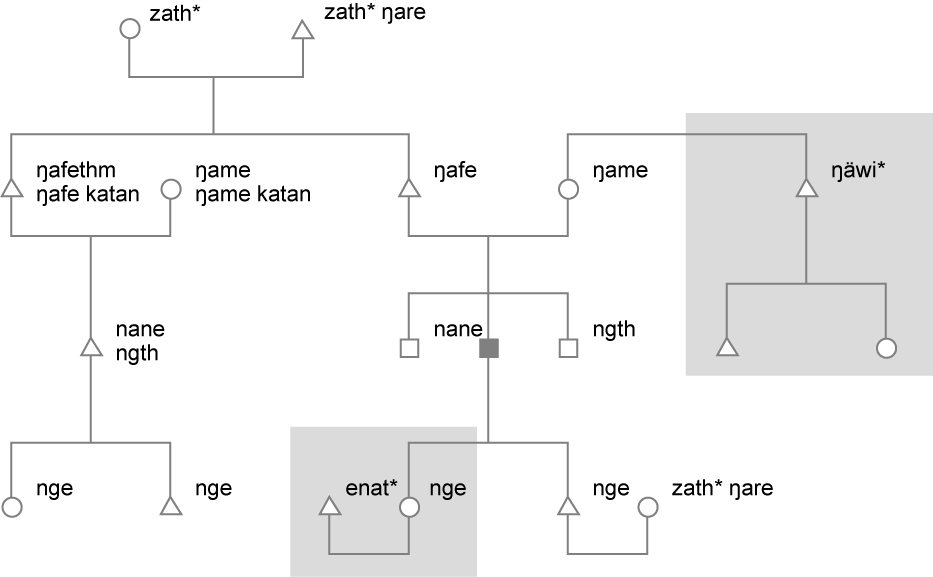
\includegraphics[width=12cm]{figures/kinship1.png}
  \caption[Consanguineal or co-resident kin terms]{Consanguineal or co-resident kin terms}\label{fig:kinship1}
\end{figure}

The spouses of ego's children are called \emph{enat} `son in-law' and \emph{zath ŋare} `daughter in-law'. Both words are used reciprocally, i.e. they mean `parents in-law' from the opposite perspective. The sex of the referent can be specified by adding \emph{ŋare}. Ayres points out that grandparents and grandchildren are equated by the same word \emph{zath}, which also means `moon' and `month', and as we have just seen `daughter in-law'. However, \emph{zath} is somewhat archaic, and the \ili{Nama} loan \emph{aki} with the same set of meanings is used in its place. Ayres explains this grouping of three meanings \textendash{} grandparents, grandchildren and daughter in-law \textendash{} by a ``structural incompleteness that is felt to be generated by the original exchange'' (\citeyear[226]{Ayres:ws}). She points out that the preferred arrangement for the daughter of an exchanged woman is to marry back to her mother's place. She concludes that the grouping of the three meanings in the same kin term encodes a cultural practise which ``assures the continuity of a man's patriline not simply through his own children, but through their children'' (\citeyear[227]{Ayres:ws}).

\begin{figure}[H]
  \centering
  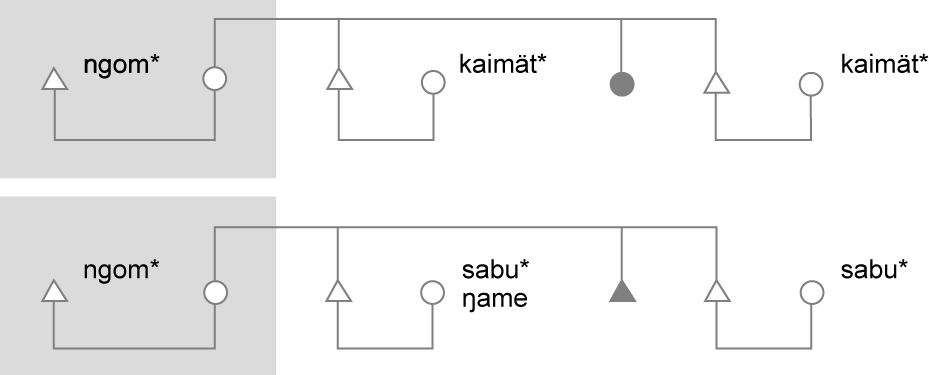
\includegraphics[width=10cm]{figures/kinship2.png}
  \caption[Same-generation, affinal kin terms for female and male ego]{Same-generation, affinal kin terms for female and male ego}\label{fig:kinship2}
\end{figure}

Figure \ref{fig:kinship2} shows the affinal kin terms in the same generation. The word \emph{ngom} `brother in-law' is used by both women and men, and for men it is used reciprocally. In (\citealt[214]{Ayres:ws}), the words \emph{ntjufaré} and \emph{nakimi} [her spelling] appear in a \isi{kinship} diagram for `brother in-law'. The former is a \ili{Kánchá} word and the latter is from Motu (\citealt[107]{Turnerlister:1935motu}). While \emph{nakimi} coexists with \emph{ngom}, \emph{ntjufare} is not used by Komnzo speakers. I suspect that this word was given to Ayres by \ili{Wára} speaking women from Yokwa. There are strong marriage ties between Rouku and Yokwa, and the process of village consolidation (\S{}\ref{modernhistory}) has led to an influx of \ili{Kánchá} speakers in Yokwa in the past. The term \emph{kaimät} is used between a woman and her brother's wife, and both are in a joking relationship. The term \emph{sabu} is used between a man and his brother's wife, and both are in a taboo relationship. The taboo is much stricter for the wife of the younger brother, who is always called \emph{sabu}. As for the wife of the older brother, one may also use \emph{ŋame} `mother' if she is sufficiently older, and the taboo relation is somewhat lax.\\

After a consummated exchange marriage, a special set of terms is used. These are shown in Figure \ref{fig:kinship3}. The word \emph{fäms} `exchange fellow' is used between the two men who have exchanged sisters, and the exchanged woman is called \emph{fäms ŋare} `exchange woman'. The children of the exchange couple are called \emph{fäŋame} or \emph{fäŋafe} depending on their sex. These two words are archaic in Komnzo and instead \emph{bäiŋame} or \emph{bäiŋafe} are used. The last vowel of both is sometimes dropped resulting in \emph{bäiŋam} or \emph{bäiŋaf}. These words are used reciprocally, but the last part (\emph{-ŋaf} and \emph{-ŋam}) encodes the sex of the referent. It is unclear when and how the first part changed from \emph{fä-} to \emph{bäi-}, but the consonants /f/ and /b/ stand in a paragidmatic relationship, because there is no voiceless counterpart of the prenasalised /b/. For this reason, I suspect that the first part is a contraction of \emph{fäms}, and \emph{fäŋame} or \emph{fäŋafe} used to be \emph{fäms ŋame} `exchange mother' and \emph{fäms ŋafe} `exchange father'. Note that the same figure can be drawn for a female ego. We would only have to change the words for wife and husband, which are \emph{fzenz} and \emph{fis} respectively.

\begin{figure}[H]
  \centering
  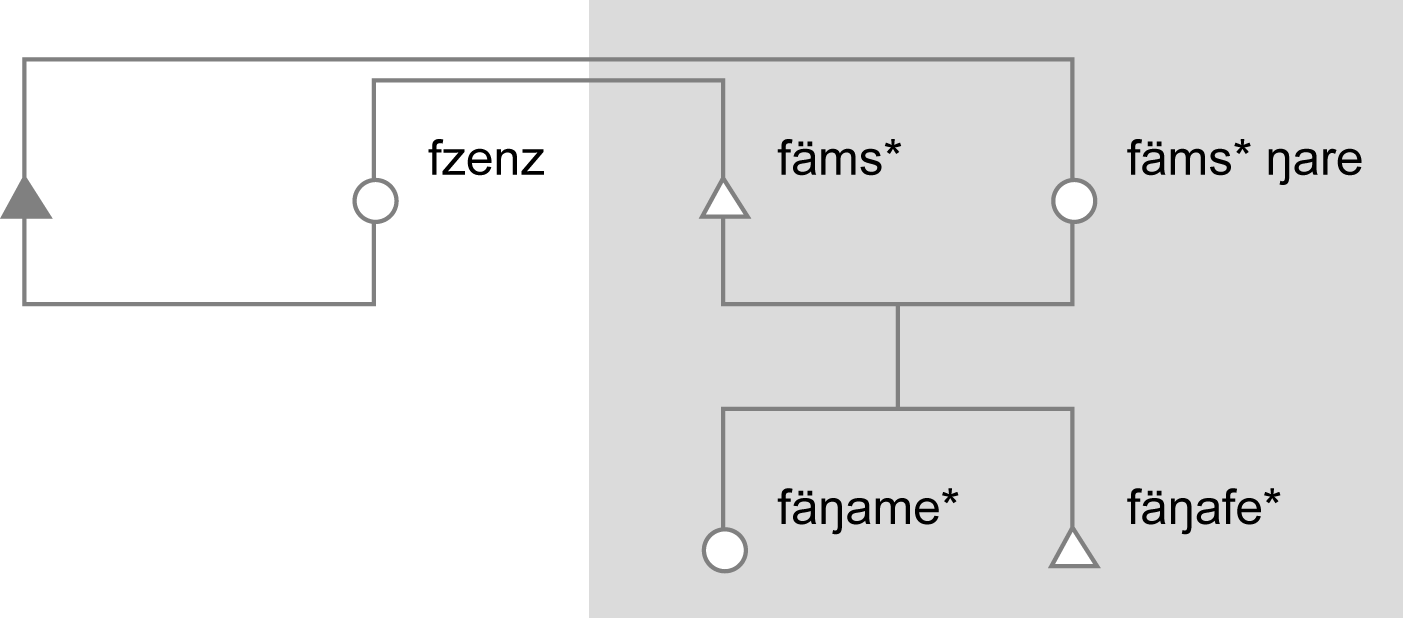
\includegraphics[width=8.5cm]{figures/kinship3.png}
  \caption[Sister-exchange kin terms: \emph{fäms}]{Sister-exchange kin terms: \emph{fäms}}\label{fig:kinship3}
\end{figure}

An exchange marriage also affects the children's generation. Ayres points out that cross-cousins are preferred marriage partners (\citeyear[217]{Ayres:ws}), but this excludes the children of an exchange. Cross-cousins from an exchange marriage refer to each other with the term \emph{yamit}. The relationship between them is more like that between siblings, which is corroborated by the fact that ego employs the same kin term \emph{ngom} for the husband of the \emph{yamit}. The wife of ego's \emph{yamit} is called \emph{yumad}. This is shown in Figure \ref{fig:kinship4}.

\begin{figure}[H]
  \centering
  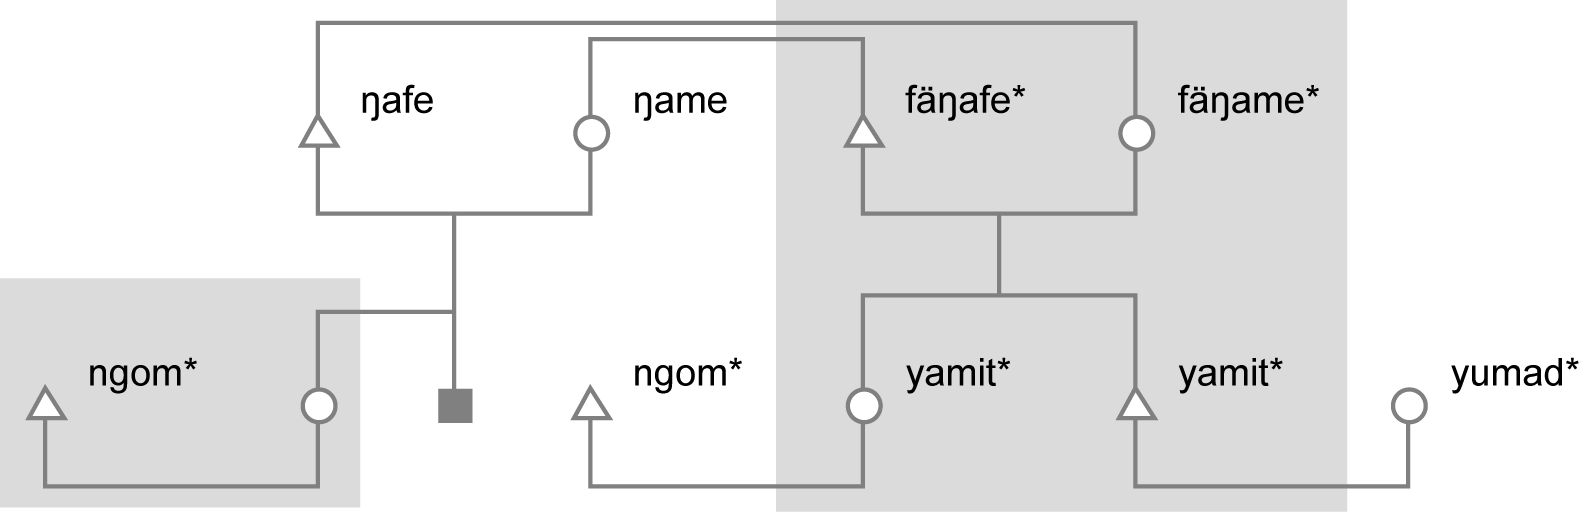
\includegraphics[width=12cm]{figures/kinship4.png}
  \caption[Sister-exchange kin terms: \emph{yamit}]{Sister-exchange kin terms: \emph{yamit}}\label{fig:kinship4}
\end{figure}

There is another special relation that holds between the affines and children of two sisters. Two men who are married to sisters refer to each other with the term \emph{nakum}. The parallel-cousins in such an arrangement refer to each other as \emph{naku}, and what holds for the \emph{yamit} relation is also true for the \emph{naku} relation. This is shown in Figure \ref{fig:kinship5}.

\begin{figure}[H]
  \centering
  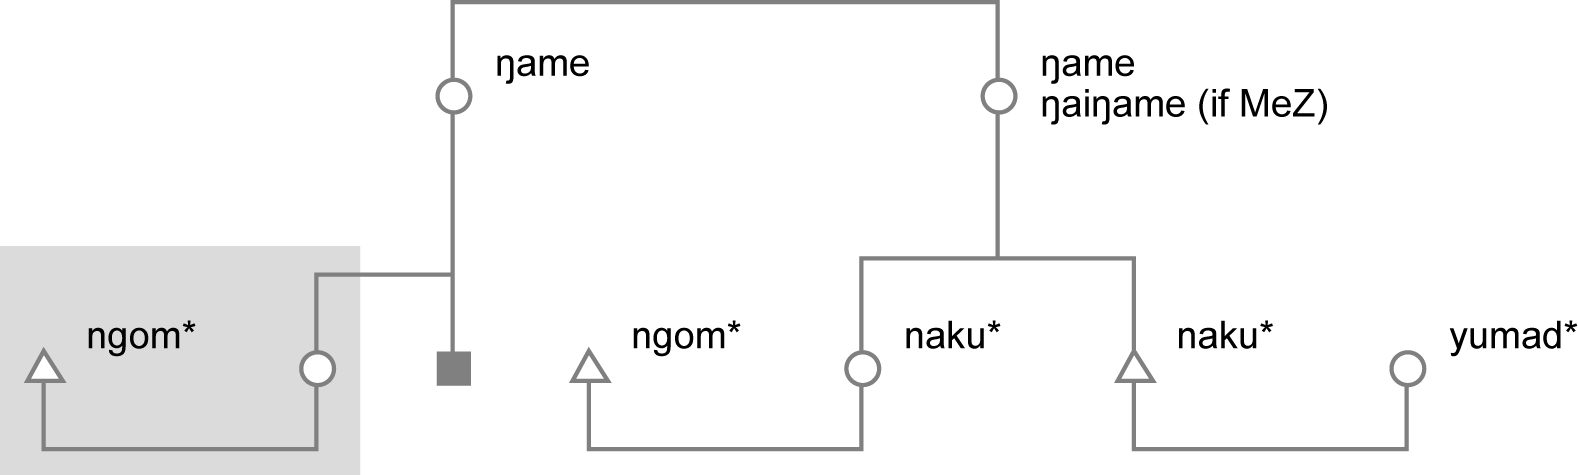
\includegraphics[width=12cm]{figures/kinship5.png}
  \caption[The \emph{naku} relationship]{The \emph{naku} relationship}\label{fig:kinship5}
\end{figure}

The rules and regulations are often explained in terms of space and Mary Ayres focusses on this aspect in her thesis. For example, informants would often explain that two individuals cannot mary because ``they come from the same place'', meaning that their mothers come from the same place in the case of a \emph{naku} relationship. But it can also mean that they result from a direct exchange between places in the case of a \emph{yamit} relationship.\\

There are other terms which function similar to kin terms. One such example is the word \emph{ngath}, which I translate as `mate'. Two children who where born around the same time are considered to be like close relatives, even if they belong to different clans and/or sections. They will grow up as close mates and they will help each other out. It is up to the parents to decide who will become \emph{ngath}, but it is always children of the same sex. I know of two cases where the \emph{ngath} relationship was inherited from the fathers who were also \emph{ngath} to each other. Another example is the word \emph{ngemäku}, which is used between the true parents of a child and the ones who have adopted the child. Adoption is very common and it occurs shortly after the weaning period. The word \emph{ngemäku} contains the word \emph{nge} `child', but the second part \emph{mäku} has no meaning by itself. A third example is the word \emph{nzäthe} `namesake'. Children are given many names when they are born. As a consequence an individual has multiple namesake relationships.\\

This section is closed with a comprehensive list of kin terms in Table \ref{kintermstable}. Alternative terms and applications as well as comments are given in the rightmost column.

{\renewcommand{\tabcolsep}{2,3pt}
\begin{longtable}{llp{3cm}p{4,7cm}}
\caption{Summary of kin terms and other relation terms}
\label{kintermstable}\\
		\lsptoprule
		\textsc{komnzo} & \textsc{gloss}&\textsc{relation}\super{a} & \textsc{comment}\\\hline
		\endfirsthead
		\textsc{komnzo} & \textsc{gloss}&\textsc{relation}\super{a} & \textsc{comment}\\\hline
		\endhead
		\emph{ŋafe} & father & F, FB & also \emph{afa} (\ili{Nama} loan)\\
		\emph{ŋame} & mother & M, MZ, FBW & also \emph{ama} (\ili{Nama} loan)\\
		\emph{nane} & brother, sister & eB, eZ & FBS and FBD (if older)\\
		\emph{ngth} & brother, sister & yB, yZ & FBS and FBD (if younger)\\
		\emph{zath} & grandparent,&FF, FM, MF, MM, & also \emph{aki} (\ili{Nama} loan),\\
		&grandchild,&SS, SD, DS, DD, &used reciprocally (rcpl.), \\
		&parent in-law,&HF, HM, SW, BSW, &can be specified for sex\\
		&daughter in-law&SSW &by adding \emph{ŋare}\\
		\emph{kaimät} & sister in-law & BW, HZ & female perspective, used rcpl.\\
		\emph{sabu} & sister in-law & BW, HB & male perspective, used rcpl.\\
		\emph{ngom} & brother in-law\super{b} & ZH, WB & also for husbands of cross-cousins\super{b}, i.e. \emph{yamit's} husband, used rcpl.\\
		\emph{yumad} & n/a & n/a & wife of parallel-cousin\super{b} (\emph{yamit's} wife), used rcpl.\\
		\emph{enat} &parent in-law& DS, WF, WM&used rcpl.\\
		&son in-law&&\\
		\emph{ŋäwi} & uncle,& MB, ZS, ZD	& also \emph{babai}, used rcpl.\\
		&niece, nephew&&\\
		\emph{fäms} & exchange\super{b}	& ZH, BW & can be specified for sex by adding \emph{ŋare}, used rcpl.\\
		\emph{fäŋame} & aunt, niece\super{b} & FZ, BD&also \emph{bäiŋam}, used rcpl.\\
		\emph{fäŋafe} & uncle, nephew\super{b} & MB, ZS&also \emph{bäiŋaf}, used rcpl.\\
		\emph{yamit} & cross-cousin\super{b} & MBS, MBD, FZS, FZD & used rcpl.\\
		\emph{naku} & parallel-cousin & MZS, MZD & used rcpl.\\
		\emph{nakum} & n/a & WZH & used rcpl.\\\hline
		\emph{thuft} & in-law & n/a & also \emph{nakimi} (Motu loan), used rcpl.\\
		\emph{ngath} & mate & n/a & between two (predetermined) mates of the same sex, used rcpl.\\
		\emph{ngemäku} & n/a & n/a & between true parent and adopted parent, used rcpl.\\
		\emph{nzäthe} & namesake & n/a & between two people with the same name, used rcpl.\\
		\lspbottomrule
		\multicolumn{4}{l}{{\footnotesize \super{a}F=father, M=mother, B=brother, Z=sister, S=son, D=daughter, H=husband, W=wife}}\\
		\multicolumn{4}{l}{{\footnotesize \super{b}only after a consummated sister exchange marriage}}\\
\end{longtable}}

\subsection{Person reference and name avoidance}\label{personref}

There is some diversity in person referring expressions in Komnzo. In the case of \isi{name avoidance}, these may be restricted to only a subset. The common expressions are: full names (given name + family name), personal names, nicknames, kin terms, other relation terms, reference via circumspection, and the \isi{recognitional} \isi{demonstrative}.\\

The \isi{kinship} system as presented above lays out a number of rules of behaviour. Amongst these is a practise of \isi{name avoidance} which holds between all affines. When recording genealogies informants would often hestitate or refuse to utter the name of a particular person and instead ask some bystander or a child to pronounce the personal name for me. Name avoidance is seen as a way of showing respect. This was explained to me by my sister while transcribing a text in which she used the personal name of her sister in-law. When I asked her, why she had not used the appropriate kin term \emph{kaimät}, she replied that she was very angry with her at the time and showed her anger by using the personal name. Name avoidance impacts on the reference to other persons with the same personal name, to whom the speaker may not be in a name-avoidance relationship. In other words, \isi{name avoidance} is independent of the referent in a particular situation. Instead \isi{name avoidance} targets the personal name. This does not result in any practical problems because people have multiple names.\\

There are different solutions to ensure that the hearer understands who is meant. In addition to the appropriate kin term, one may use circumspection or a \isi{recognitional} \isi{demonstrative}. For example, the name of one of my brothers in-law is \emph{Kurai}. I should not utter his name, but use the kin term \emph{ngom} instead. In many situations, this term is sufficient to establish the correct reference. Alternatively, I can use circumspection strategy like \emph{tokoafis} `Toko's husband' or a teknonym \emph{weweaŋafe} `Wewe's father'. For teknonyms, it is usually the name of first-born child that is used, regardless of sex. A third solution, is to use the \isi{recognitional} \isi{demonstrative}. The \isi{recognitional} \isi{demonstrative} can be roughly translated to \ili{English} as `the one that we both know about' (see \S\ref{recognitional-pronoun}).\\

The different strategies of \isi{person reference} can be ranked according to how much knowledge is presupposed on the part of the hearer. For example, a personal name requires very little contextual knowledge, whereas a \isi{recognitional} \isi{demonstrative} requires much more. We may rank these strategies like this: full name (\emph{Kurai Tawth}) > personal name (\emph{Kurai}) > circumspection/teknonym (\emph{tokoafis} `Toko's husband') > kin term (\emph{ngom} `brother in-law') > \isi{recognitional} (\emph{baf} `that one'). Note that using a full name is a recent adaptation to western culture, which is only employed in the context of a census or some other administrational matter. It is a common practise in PNG to use the name of the father as family name. Hence, \emph{Kurai's} father was \emph{Tawth} and therefore his full name is \emph{Kurai Tawth}. In daily interaction, this strategy is absent.\\

A person has a multitude of personal names or nicknames. Almost everyone has a set of five to ten names and the frequency of use of any one of these may come and go like a fashion. Shortly after birth, or sometimes even before birth, different relatives will propose names for the new-born. These may be their own names, which establishes a namesake relationship. In fact, the word \emph{nzäthe} `namesake' is the most frequent term of address. There is a special ceremony a couple of months after birth, where the name-giver presents gifts to his namesake and holds the baby for the first time. Names may also be created on the spot, as nicknames or as self-attributions. For example, the three elders of the \emph{Mrzar Mayawa} clan in Rouku are \emph{Marua}, \emph{Kaumb} and \emph{Abia}. Their respective nicknames are \emph{oroman loŋ} `old man long' because he prefers wearing long trousers, \emph{afa kwanz} `father bald head' because he is bald and \emph{afa thwä} `father catfish' because he has a big belly. The first of them, \emph{Marua}, decided one day that he should be called \emph{oroman zulai} `old man july'. To my bewilderment, I found that everyone had accepted this name within a few weeks. Interestingly, a namesake relationship may transfer all of these names to the namesake. For example, a small baby boy was given the name \emph{Marua}, thus establishing a namesake relationship. Today, the toddler is sometimes called \emph{Marua}, \emph{loŋ} or \emph{zulai}.

\subsection{Language ideology and multilingualism}\label{ideomulti}

Language ideology is characterised by a set of beliefs on the part of speakers about the role which language plays in constructing their social world (\citealt{Silverstein:1979li}, \citealt{Rumsey:1990vb} and \citealt{Makihara:2007co}). In the Morehead Region, people draw a strong connection between land and speech variety. This native linguistic ideology is similar to Aboriginal cultures, especially in Arnhem Land (\citealt{Merlan:1981ue}) and Cape York (\citealt{Sutton1978:ws}). As for the Farem people, this ideology surfaces through open statements and explanations, the expected behaviour of in-marrying women, ancestor stories, but it is also entailed in metaphors. I will briefly note some of my own observations on \isi{language ideology} here.\\

In Rouku, there is strong social pressure on all members of the community to speak Komnzo. This is openly expressed during public speeches, but also by individuals in conversation or during interviews. One often hears that women should not talk in `their language' to the children, but in Komnzo. In practice, this is often violated and virtually everybody grows up in a \isi{multilingual} context. We can take an example which is the result of the process of village consolidation described in \S\ref{modernhistory}. A number of older men originally from Rouku have stayed for a long time in \ili{Anta} or \ili{Wára} speaking villages, and consequently their children grew up with those varieties as their main language. The children, now in their late 40's, have moved back to Rouku. Some of them have married a woman from their natal villages and hence the dominant language of some Farem households is \ili{Anta} or \ili{Wára}. However, when I administered a socio-linguistic questionaire, they would deny speaking anything but Komnzo.\\

In an attempt to understand the situation, I conducted sociolinguistic interviews with about 40 people. Amongst the questions were some which targeted \isi{language ideology} (``What is your language?'', ``What do think about language mixing in the village?'', ``What language do you want your children to learn?''). The conclusion from these interviews is that language and land form an inseparable bond. I defer the statistical analysis of the interviews to another point in time. The bond between language and land is identical to the bond between a group of people and their origin place. This bond is transmitted through the father's line. An example taken from the interviews is that of an older woman who lives in Rouku. She explained to me that she grew up in Yokwa, and consequently she speaks \ili{Wára} most of the time. Although she speaks mostly \ili{Wára}, she knows that this is not the language of the place. She wishes for her children to speak Komnzo. When asked about `her language' she answered \ili{Kánchá} instead of \ili{Wára}. She explained that her father had moved as a teenager from a \ili{Kánchá} speaking village to Yokwa. It follows that regardless of whether an individual uses predominantly mother's language or the language of the village, he or she will identify with the language of his or her father's place.\\

Mixing or shifting languages, although very common, is almost universally looked down upon. The answers as to why this behaviour is thought of as inappropriate often follow along the lines of matching language to place (``They should not speak \ili{Wára} here because this is the language of Yokwa'', ``We should not mix languages because the children will not be able to name the places and animals that belong to our land'').\\

Women who marry in are expected to shift to the local language, but this is often not followed because there are enough women from any one village to form small exclaves, for example of \ili{Wára} speaking women in Komnzo speaking territory. It is hard to corroborate, but informants say this was enforced more in the past. For example, there are spells and rituals to enhance the language learning process on the side of the woman. One ritual involves splitting a thin bamboo behind a woman's head and whispering a spell. This procedure is said to facilitate the learning process. I asked many times to have this procedure performed on me, but people refused to do it because I would forget my native \ili{German}. There are other customs and rules which connect land and language. For example, it is forbidden to talk another language at story places and men would introduce their new bride to a \textit{menz} `story man' at a particular place in order to avoid sickness. The policy of language shift expected from women is hardly ever enforced these days and one might wonder whether it ever was. Ayres (\citeyear[226]{Ayres:ws}) describes the preference for a daughter to marry back into her mother's village, which she calls a short marriage cycle. This pattern establishes strong ties between particular villages. In the case of the Rouku it is the village of Yokwa and the language is \ili{Wára}. As mentioned above, groups of women from Yokwa would often speak \ili{Wára} between themselves or to their children and there is no reason why this should have been different in the past. But when asked about this, they would look down on `language mixing' and stress the importance of the correct language at the right place.\\

Ancestor stories almost always involve comments on language. For example, the Kuramonggo myth which is found across the Morehead Region involves an ancestor who heard voices coming from a tree. Different versions are found in (\citealt[299]{Williams:1936transfly}) and (\citealt[102]{Ayres:ws}). In the myth, the ancestor starts to chop the tree into segments from the top to the bottom. With each little bit that he chopped, people speaking different languages came out and started running towards their respective places. The further he worked his way to the bottom of the tree, the more intelligible the words became to him. When he reached the base of the tree, he heard his own language and thus his own people emerged from the tree. A common \isi{metaphor} that explains the language situation from a local perspective builds on this story. One often hears the local language being described as \emph{zfth} `the base of a tree' and all the surrounding languages as \emph{tuti} `the branches'. The tree \isi{metaphor} is important in the local perspective. For example, women are jokingly described as \textit{bidr} `flying foxes' because they fly from tree to tree, and sometimes they are described as \textit{fätü} `a wild yam' or \textit{saka} `mustard vine' because the vines of these plants grow on trees.

\section{Komnzo within the Yam languages}\label{Komnzowithinyam}

This section situates Komnzo within the \ili{Yam languages}. This language family was formerly referred to as the ``Morehead and Upper Maro Rivers languages'', or ``\ili{Morehead-Maro} languages'' (\citealt{Wurm:1971uw}). This name is misleading because its geographical boundary in the east, the Morehead River, excludes all the languages of the \ili{Nambu} subgroup. I follow Evans in using the more precise term ``\ili{Yam languages}'' (\citeyear[124]{Evans:2012wp}). Not only are yams the staple food, and of high cultural importance in exchange feasts, they also gave rise to the \isi{senary} \isi{numeral system}, which is unique to the languages of the family. In addition to the \ili{English} word yam [jæm], the word \emph{yam} [jam] carries high cultural significance in many \ili{Yam languages}. For example, in Komnzo it means `footprint, custom, tradition' and in \ili{Nen} it means `law, tradition, culture'.\\

The \ili{Yam languages} comprise three subgroups: \ili{Nambu} in the east, \ili{Tonda} in the west, and Yei, which has only a single member. A first attempt to reconstruct various aspects of the proto language can be found in (\citealt{Evans:sng}). While it is relatively easy to place Komnzo in the \ili{Tonda} subgroup, it is much harder to classify the units within \ili{Tonda}; in other words to draw a boundary between language and dialect. Are Komnzo, \ili{Anta} and Wérè dialects of \ili{Wára} as Ethnologue\footnote{URL: \href{http://www.ethnologue.com/language/tci}{http://www.ethnologue.com/language/tci}} portrays it or are they languages in their own right? Peter Mühlhäusler (\citeyear{Muhlhausler:2006naming}) points out the difficulty and futility in answering such questions in Papua New Guinea and the contradictions that different researchers have produced in the past. As the preceding description of \isi{language ideology} has highlighted, these are considered to be different languages from a local perspective. I remain agnostic throughout this section and offer a short conclusion at the end.\\

I discuss sound correspondences and sound changes first. Next, I show some lexicostatistic data from (\citealt{Wurm:1971uw}) and (\citealt{Clifton:1991fly}). Last, I discuss case markers, pronouns and verb morphology. I include here the following \ili{Tonda} varieties: Komnzo, \ili{Anta}, \ili{Wára}, \ili{Wèré}, \ili{Ránmo}, \ili{Blafe}, \ili{Wartha} Thuntai and \ili{Kánchá}. I refer the reader to Figure \ref{moreheadmap} for an overview where these varieties are spoken. I do not include \ili{Arammba}, which I take to be sufficiently different to be considered a separate language (\citealt{Bouve:2003ar}). I have no data for the \ili{Tonda} varieties spoken on the Indonesian side of the border (Baedi, \ili{Ngkolmpu}, Smerky, Bakari, Taemer and Sota), and only very little data on \ili{Kémä}.\\

With the exception of Komnzo, the spelling of the names of these varieties is adopted from Ethnologue, which in turn goes back to an \isi{orthography} workshop held by SIL missionaries in Morehead in 2000. Note that the orthographies were developed for each variety with the result that the graphemes in the language names have different phonetic values: Komnzo [kɞ̆m\super{n}dʒo], \ili{Anta} [a\super{n}da], \ili{Wára} [wæra], \ili{Wèré} [wɞ̆rɛ], \ili{Ránmo} [rænmo], \ili{Blafe} [\super{m}blæɸe], \ili{Wartha} Thuntai [warða ðu\super{n}da͡ı], \ili{Kánchá} [kə̆\super{n}dza]. To ensure comparability in this section, I will employ IPA for all language examples, including Komnzo.

\subsection{Phonology}\label{comp-phon}

First, I turn to phonological correspondences. In this section, the languages in the tables are sorted geographically: west (left) to east (right). We find that only \ili{Blafe} and \ili{Ránmo} have an /l/ phoneme in their respective inventories. Table \ref{lth} shows that this phoneme corresponds to an interdental fricative in Komnzo, \ili{Anta}, \ili{Wára}, \ili{Wèré}, \ili{Wartha} Thuntai and \ili{Kánchá}. Note that final \isi{devoicing} produces [θ] in coda position.

\begin{table}[H]
\caption{Correspondence set: [l] versus [ð]}
\label{lth}
	\begin{tabular}{llp{1,3cm}p{1,3cm}lllp{1,5cm}}
		\lsptoprule
		&\textsc{item} &Blafe, Ránmo &Wartha Thuntai &Kánchá &Wèré &Anta &Komnzo, Wára \\\hline
		1 &\textsc{tongue} &læmin &ðæmin &ðæmin &ðæmin &ðæmin &ðæmin\\
		2 &\textsc{excretes} &wəl &wəθ &wəθ &wəθ &wəθ &wəθ\\
		3 &\textsc{wet} &kilkil &kiθkiθ &tʃiθtʃiθ &tiθtiθ &tiθtiθ &tʃiθtʃiθ\\
		4 &\textsc{armpit} & \super{ŋ}gəlki &\super{ŋ}gəθki &kəθtʃi &\super{ŋ}gəθki &\super{ŋ}gəθtʃi &\super{ŋ}gəθtʃi\\
		\lspbottomrule
	\end{tabular}
\end{table}%Correspondence set: [l] versus [ð]

A second set shows the correspondence of bilabial stops, [\super{m}b] and [b], in \ili{Blafe}, \ili{Ránmo} and \ili{Wartha} Thuntai to lavio-\isi{velar} stops, [\super{ŋ}g\super{w}] and [k\super{w}], in Komnzo, \ili{Anta}, \ili{Wára}, \ili{Wèré} and \ili{Kánchá} in Table \ref{mbng}. We find that the labial part is sometimes realised as a rounded back vowel, [\super{ŋ}go] and [ko], in \ili{Kánchá}, \ili{Wèré} and \ili{Wartha} Thuntai, for example in lines 3 (`butterfly') and 4 (`crow'). One possible explanation is a process of develarisation that has occurred in \ili{Blafe}, \ili{Ránmo} and \ili{Wartha} Thuntai.

\begin{table}[H]
\caption{Correspondence set: [\super{m}b/b] versus [\super{ŋ}g\super{w}/k\super{w}]}
\label{mbng}
	\begin{tabular}{llp{1,5cm}p{1,5cm}llp{1,5cm}}
		\lsptoprule
		&\textsc{item} &Blafe, Ránmo & Wartha Thuntai & Kánchá& Wèré &Komnzo, Wára, Anta\\\hline
		1 &\textsc{nest} &\super{m}bəl &\super{m}bəθ &\super{ŋ}g\super{w}əθ	&\super{ŋ}g\super{w}əθ &\super{ŋ}g\super{w}əθ\\
		2 &\textsc{mosquito} &\super{m}bæ &\super{m}bæ &\super{ŋ}g\super{w}æ &\super{ŋ}g\super{w}æ &\super{ŋ}g\super{w}æ\\
		3 &\textsc{butterfly} &ta\super{m}bam &ta\super{m}buram &\super{m}bæ\super{ŋ}goram &\multicolumn{2}{c}{\super{m}bæ\super{ŋ}g\super{w}ərəm}\\
		4 &\textsc{crow} &\super{m}baθ &kot &koθ &koθ &k\super{w}aθ\\
		5 &\textsc{light} &praja &bæjan &k\super{w}ajan &k\super{w}ajan &k\super{w}ajan\\
		6 &\textsc{sick} &bik &bik &k\super{w}ik &k\super{w}ik &k\super{w}ik\\
		\lspbottomrule
	\end{tabular}
\end{table}%Correspondence set: [\super{m}b/b] versus [\super{ŋ}g\super{w}/k\super{w}]

There is a small set of words in which the bilabial fricative corresponds to a prenasalised bilabial stop. The set in Table \ref{fmb} groups again \ili{Blafe}, \ili{Ránmo} and \ili{Wartha} Thuntai against Komnzo, \ili{Anta}, \ili{Wára}, \ili{Wèré} and \ili{Kánchá}. Interestingly, the form of the \Second\Sg.\Abs{} `you' groups \ili{Blafe}, \ili{Ránmo}, \ili{Wartha} Thuntai, \ili{Kánchá} and Komnzo together.

\begin{table}[H]
\caption{Correspondence set: [\super{m}b] versus [ɸ]}
\label{fmb}
 	\begin{tabular}{llp{1,5cm}p{1,5cm}p{1,5cm}p{2cm}}
 		\lsptoprule
 		&\textsc{item}& Blafe, Ránmo & Wartha Thuntai &Kánchá, Komnzo & Wára, Anta, Wèré\\\hline
 		1 &\textsc{wife} &\super{m}bə\super{ŋ}ge\super{n}t &\super{m}bə\super{ŋ}ge\super{n}ts &ɸətʃe\super{n}ts &ɸətʃe\super{n}ts\\
 		2&\textsc{husband} &\super{m}bi &\super{m}bi &ɸis &ɸis\\
 		3&\Second\Sg.\Abs{} `you' &\super{m}bæ &\super{m}bæ &\super{m}bæ &ɸe\\
 		\lspbottomrule
 	\end{tabular}
\end{table}%Correspondence set: [\super{m}b] versus [ɸ]
\vspace{-.4cm}
A clear \isi{directional} change is palatalisation before front vowels. In Table \ref{palatal}, I show only a subset of the varieties. Komnzo represents those in which palatalisation has occured. This holds also true of \ili{Anta} and \ili{Wára}, but the forms are slightly different. \ili{Wartha} Thuntai represents those in which palatalisation has not occured. This is also the case in \ili{Blafe} and \ili{Ránmo}. The table shows that \ili{Wèré} and \ili{Kánchá} are somewhat irregular. In lines 4 and 5 (`house' and `one') palatalisation occurs in \ili{Wèré}, but not in \ili{Kánchá}. Line 6 (`armpit') shows the opposite. In lines 1-3 (`woman', `I', `people') palatalisation has occured in both and in line 7 (`tree') in neither. I have included \ili{Nama}, a \ili{Nambu} language, to show that \ili{Nambu} languages preserve the original \isi{velar} quality, for example in lines 1, 3, and 4 (`woman', `people', `house'). Note that in line 5 (`one'), \ili{Nambu} has dropped the first consonant. The deletion of initial \isi{velar} \isi{nasals} is a regular change in \ili{Nambu} languages, for example `mother' is [ŋame] in Komnzo, but [ama] in \ili{Nama} and \ili{Nen}. Note that the conditioning context for palatalisation has been lost in line 4 (`house'), because the examples end in a consonant. \ili{Nama} attests a vowel in this position.

\begin{table}[H]
\caption{Palatalisation before front vowels}
\label{palatal}
	\begin{tabular}{llp{1,5cm}llll}
		\lsptoprule
			&\textsc{item} & Wartha Thuntai	&Kánchá &Wèré &Komnzo &Nama\\\hline
			1 &\textsc{woman}\super{a} &\super{m}broki &\super{m}brotʃi &\super{m}brasi &\super{m}bratʃi &\super{m}brake\\
			2 &\Fsg.\Abs &\super{ŋ}ga &\super{n}dʒæ &se &\super{n}dʒæ &(jə\super{n}d)\\
			3 &\textsc{people}\super{b} &\super{ŋ}gʏ\super{n}təm &tʃœ\super{n}təm &sœ\super{n}tmæ &tʃœ\super{n}tmæ &\super{ŋ}gʏ\super{n}tmæ\\
			4 &\textsc{house} &me\super{n}k &mə\super{ŋ}k &mə\super{n}ts &mə\super{n}ts &mæ\super{ŋ}go\\
			5 &1 (\textsc{one}) &ŋæ\super{m}bi &ŋæ\super{m}bi &næ\super{m}bi &næ\super{m}bi &æ\super{m}biro\\
			6 &\textsc{armpit} &\super{ŋ}gəθki &kəθtʃi &\super{ŋ}gəθki &\super{ŋ}gəθtʃi &-\\
			7 &\textsc{tree type} &\super{ŋ}gœ\super{n}t &\super{ŋ}gœ\super{n}t &\super{ŋ}go\super{n}t &\super{n}dʒœ\super{n}ts &-\\
		\lspbottomrule
		\multicolumn{7}{l}{\footnotesize{\textsuperscript{a}a woman in the time after giving birth}}\\
		\multicolumn{7}{l}{\footnotesize{\textsuperscript{b}people who live to the west of one's own group}}\\
		%\multicolumn{7}{l}{\footnotesize{\textsuperscript{c}Terminalia megalocarpa}}\\
	\end{tabular}
\end{table}%Palatalisation before front vowels

The last set shows the correspondence between stops and affricates. In Table \ref{affrstop}, \ili{Blafe}, \ili{Ránmo}, \ili{Wèré} and \ili{Anta} are grouped against Komnzo, \ili{Wára}, \ili{Wartha} Thuntai and \ili{Kánchá}.

\begin{table}[H]
\caption{Correspondence set: stop versus affricate}
\label{affrstop}
	\begin{tabular}{llp{1,1cm}p{1,3cm}lllp{1,3cm}}
		\lsptoprule
		&\textsc{item} &Blafe, Ránmo &Wartha Thuntai &Kánchá &Wèré &Anta &Komnzo, Wára\\\hline
		1 &\textsc{pain} &ti &\super{n}dʒi &tʃi &ti &ti &tʃi\\
		2 &\textsc{right} &tawe &tsowe &tsowe &tawe &tawe &tsawe\\
		3 &\textsc{bowerbird} &\super{n}dojar &\super{n}dʒojar &\super{n}dʒojar &\super{n}dʒojar &\super{n}dojar &\super{n}dʒœjar\\
		\lspbottomrule
	\end{tabular}
\end{table}%Correspondence set: stop versus \isi{affricate}

Concluding the comparison of phonological correspondences, we find that Komnzo and \ili{Wára} are almost always grouped together, and we may include \ili{Anta} as well. \ili{Kánchá} and \ili{Wèré} share a number of correspondences with Komnzo, \ili{Wára} and \ili{Anta}, but they differ in some sets. \ili{Blafe}, \ili{Ránmo} and \ili{Wartha} Thuntai are different in almost all sets. While \ili{Blafe} and \ili{Ránmo} are always grouped together, \ili{Wartha} Thuntai can be grouped with the other varieties in some sets.

\subsection{Lexicon}\label{comp-lex}

In this section, I present data from (\citealt{Wurm:1971uw}) and (\citealt{Clifton:1991fly}). I defer the statistical analysis of my own wordlists to a latter point in time.\\

A first calculation of cognate rates was offered by Wurm. His dataset comprised \ili{Tonda} and \ili{Nambu} languages as well as and Yei and \ili{Marori}. In Table \ref{wurm1971} only the \ili{Tonda} varieties have been extracted. Wurm's language labels refer to different \ili{Tonda} varieties: Upper Morehead (Komnzo, \ili{Wára}, \ili{Anta}, \ili{Arammba}), Lower Morehead (\ili{Kánchá}), \ili{Tonda} (\ili{Blafe}, \ili{Ránmo}, \ili{Wartha} Thuntai, \ili{Wèré}) and \ili{Kanum} (Baedi, \ili{Ngkolmpu}, Smerky, Bakari, Taemer, Sota).

\begin{table}[H]
\caption[Cognate rates]{Cognate rates (adopted from \citealt[159]{Wurm:1971uw})}
\label{wurm1971}
	\begin{tabular}{|c|c|c|c|}
		\cline{1-1}
		Upper Mhd 	& \multicolumn{3}{c}{} \\ \cline{1-2}
		71\% 		& Lower Mhd &  \multicolumn{2}{c}{} \\ \cline{1-3}
		60\% 		& 55\% 		& \ili{Tonda} 	&  \multicolumn{1}{c}{} \\ \cline{1-4}
		39\% 		& 39\% 		& 40\% 		& \ili{Kanum}\\ \cline{1-4}
	\end{tabular}
\end{table}

A more fine-grained dataset comes from a SIL survey conducted by Clifton, Dyall and O'Rear (\citeyear{Clifton:1991fly}), who collected wordlists in 18 villages of both \ili{Tonda} and \ili{Nambu} languages. In Table \ref{clifton1991}, I show only the \ili{Tonda} varieties, but I exclude \ili{Arammba}, Rema and \ili{Kémä}, and I choose Bondobol as the village representative of \ili{Kánchá}. Moreover, I have rearranged their data in order to present the varieties geographically from west to east.

\begin{table}[H]
\caption[Rates of shared vocabulary]{Rates of shared vocabulary (extracted from \citealt{Clifton:1991fly})}
\label{clifton1991} \vspace{.3cm}
	\begin{tabular}{|c|c|c|c|c|c|c|c|}
		\cline{1-1}
		\ili{Blafe}& \multicolumn{7}{c}{} \\ \cline{1-2}
		80\% &\ili{Ránmo}& \multicolumn{6}{c}{} \\ \cline{1-3}
		63\% & 59\% &\ili{Wartha}& \multicolumn{5}{c}{} \\ \cline{1-4}
		32\% & 40\% & 52\% &\ili{Kánchá}& \multicolumn{4}{c}{} \\ \cline{1-5}
		49\% & 55\% & 55\% & 59\%&\ili{Wèré}& \multicolumn{3}{c}{} \\ \cline{1-6}
		43\% & 51\% & 50\% & 70\%& 84\%&\ili{Wára}& \multicolumn{2}{c}{} \\ \cline{1-7}
		44\% & 51\% & 50\% & 61\%& 72\%& 82\%&\ili{Anta}& \multicolumn{1}{c}{} \\ \cline{1-8}
		41\% & 49\% & 46\% & 70\%& 72\%& 87\%& 88\%&Komnzo\\ \cline{1-8}
	\end{tabular}
\end{table}

My own wordlists confirm the data in Table \ref{clifton1991}. We can draw some conclusions: (i) \ili{Blafe} and \ili{Ránmo} can be grouped together, (ii) \ili{Wartha} Thuntai is different from all other varieties, (iii) Komnzo, \ili{Wára} and \ili{Anta} can be grouped together, (iv) \ili{Wèré} and \ili{Kánchá}, though different from each other, are close to Komnzo, \ili{Wára} and \ili{Anta}. If we compare these statements to the map in Figure \ref{moreheadmap}, we find that the rates of shared vocabulary between Komnzo, \ili{Wára}, \ili{Anta}, \ili{Wèré} and \ili{Kánchá} roughly reflect geography. As for \ili{Blafe}/\ili{Ránmo} and \ili{Wartha} Thuntai, this cannot be said. In other words, if we try to understand the relation of these varieties as a dialect chain, we would have to make two cuts. The first cut splits off \ili{Blafe} and \ili{Ránmo}. The second cut singles out \ili{Wartha} Thuntai, while the remaining varieties belong to a single dialect chain.

\subsection{Morphosyntax}\label{comp-morph}

As an intermediate summary, we can conclude that Komnzo, \ili{Anta}, \ili{Wára}, \ili{Wèré} and \ili{Kánchá} are somewhat closer together as opposed to \ili{Blafe}, \ili{Ránmo} and \ili{Wartha} Thuntai. Therefore, I will focus on the first group in this section.\\

Table \ref{compcase} shows a comparison of case markers. We find that Komnzo deviates from the other varieties in the ergative singular and non-singular, and in the allative. \ili{Kánchá} deviates from the others in the ablative and the locative for consonant final words.

\begin{table}[H]
\caption{Comparison of case markers}
\label{compcase}
 	\begin{tabular}{llllll}
		\lsptoprule
 		& \ili{Kánchá} &\ili{Wèré} &\ili{Wára} &\ili{Anta} &Komnzo \\\hline
 		\Erg.\Sg&-o&-o&-o&-o&-ɸ\\
		\Erg.\Nsg&-oi&-ai&-əı&-əı&-jə\\
		&&&&&\\
		\All&-ɸ&-ɸ&-ɸ&-ɸ&-ɸo\\
		\Abl&-ɸo&-ɸa&-ɸa&-ɸa&-ɸa\\
		&&&&&\\
		\Loc{} V\_&-n&-n&-n&-n&-n\\
		\Loc{} C\_&-i&-en&-en&-en&-en\\
		\lspbottomrule
	\end{tabular}
\end{table}
\vspace{-.3cm}
Table \ref{comp-pron} shows a comparison of free pronouns. We find that Komnzo and \ili{Kánchá} share an number of forms or some element of a form. For example the first consonant of the first and second \isi{person} in both \isi{absolutive} and \isi{ergative} case. In the \isi{possessive} non-singular pronouns, only Komnzo and \ili{Kánchá} attest a separate element which signals \isi{non-singular} \emph{-me} in addition to the vowel change found in all varieties. However, the first consonant of the third \isi{person} \isi{ergative} and \isi{possessive} pronouns differs only in \ili{Kánchá}.\\

As the last topic in this section, I briefly address the marking of \isi{dual} \isi{number}. In Komnzo as in most \ili{Yam languages}, \isi{dual} \isi{number} is marked on the \isi{verb}. The affix encodes \isi{dual} versus \isi{non-dual} \isi{number}, and its value has to be integrated with information from other morphological sites to yield the three \isi{number} values \isi{singular}, \isi{dual} and \isi{plural}. I address this topic in \S\ref{dualextrs} and \S\ref{numbersubsec}. For now, it is sufficient to compare the site of \isi{dual} marking on the \isi{verb}. In some varieties this depends on the type of \isi{verb} stem which is employed. Most verbs have two stems which are sensitive to \isi{aspect}. While multiple \isi{verb} stems are attested in all \ili{Tonda} varieties, the encoding of duality differs. In Komnzo, \ili{Anta}, \ili{Wára} and \ili{Kánchá}, there are two options: duality is encoded in a suffix if the `\isi{extended stem}' is used, but in a prefix if the `\isi{restricted stem}' is used. The meaning of these labels in Komnzo is explained in \S\ref{roots-and-temp}. Only in \ili{Wèré}, duality is always encoded in a suffix regardless of the type of stem. \ili{Blafe}, \ili{Ránmo} and \ili{Wartha} Thuntai have lost \isi{dual} marking on both stem types. In these three varieties, \isi{dual} marking occurs only in high frequency verbs such as the copula or the verb `walk', where it is usually suppletive. I sketch out a tentative historical explanation of this in \S\ref{comparativenoteextrs}.

\begin{table}[H]
\caption{Comparison of free pronouns}
\label{comp-pron}
	\begin{tabular}{lllllll}
		\lsptoprule
 		& &\ili{Kánchá} &\ili{Wèré} &\ili{Wára} &\ili{Anta} &Komnzo \\\hline
		\multirow{4}{*}{\Abs}&\Fsg&\super{n}dʒæ&se&tʃe&tʃe&\super{n}dʒæ\\
		&\Fnsg&ni&ni&ni&ni&ni\\
 		&\Second&\super{m}bæ&ɸe&ɸe&ɸø&\super{m}bæ\\
		&\Third&ɸi&ɸi&ɸi&ɸi&ɸi\\
		&&&&&&\\
		\multirow{6}{*}{\Erg}&\Fsg&\super{n}dʒən&sən&tsən&tsən&\super{n}dʒe\\
		&\Fnsg&nin&ni&ni&ni&ni\\
 		&\Ssg&\super{m}bən&ɸən&ɸən&ɸən&\super{m}be\\
		&\Snsg&\super{m}bən&ɸe&ɸən&ɸən&\super{m}bənə\\
 		&\Tsg&tʃaɸ&naɸo&naɸo&naɸo&naɸ\\
		&\Tnsg&tʃaɸ&naɸ&naɸ&naɸ&naɸa\\
		&&&&&&\\
		\multirow{6}{*}{\Poss}&\Fsg&\super{n}dzuni&\super{n}done&\super{n}dzone&\super{n}done&\super{n}dzon\\
		&\Fnsg&\super{n}dʒenme&\super{n}dane&\super{n}dzane&\super{n}dane&\super{n}dʒenme\\
		&\Ssg&\super{m}buni&\super{m}bone&\super{m}bone&\super{m}bone&\super{m}bone\\
		&\Snsg&\super{m}benme&\super{m}bane&\super{m}bane&\super{m}bane&\super{m}benme\\
 		&\Tsg&tʃaɸani&naɸəne&naɸəne&naɸəne&naɸane\\
		&\Tnsg&tʃaɸanme&naɸane&naɸane&naɸane&naɸanme\\
 		\lspbottomrule
	\end{tabular}
\end{table}

\subsection{Summary}\label{comp-sum}

In conclusion, we may say that the different levels of comparision converge. Sound correspondences, lexicostatistics are well as morphological differences single out at least three separate units: \ili{Blafe}/\ili{Ránmo}, \ili{Wartha} Thuntai and a chain of dialects, which we may call `Eastern \ili{Tonda}'. The latter comprises \ili{Wèré}, \ili{Wára}, \ili{Kánchá}, \ili{Anta}, Komnzo and probably \ili{Kémä}. Eastern \ili{Tonda} shows characteristics which are typical of dialect chains: geographically distant varieties, for example Komnzo and \ili{Wèré} or \ili{Anta} and \ili{Kánchá}, show the biggest differences. Close neighbours, on the other hand, like Komnzo and \ili{Wára} or \ili{Anta} and \ili{Wèré} are very similar. That being said, I will remain cautious until more data has been gathered, and I will continue to refer to all of them as varieties. In this way, I pay respect to the native linguistic ideology which picks up on the slightest differences as being highly emblematic markers of socio-linguistic identity.

\section{Previous work and methodology}\label{prevmethod}

\subsection{Previous work}\label{previouswork}

There has been no previous research on Komnzo that goes beyond the collection of wordlists. One example is the SIL survey discussed in the preceding section (\citealt{Clifton:1991fly}). The activity of SIL missionaries in the area has led to a number of \isi{orthography} worksheets, unpublished manuscripts, surveys or theses. Examples of work on the surrounding varieties are: a grammatical sketch of \ili{Arammba} (\citealt{Bouve:2003ar}), a thesis on \ili{Wára} verb morphology (\citealt{Sarsa2001:wa}) and a socio-linguistic survey of the \ili{Tonda} subgroup (\citealt{Grummit:2012sur}).\footnote{I have written a review of the survey, which can be found under the following URL: \href{https://www.researchgate.net/publication/266079354}{https://www.researchgate.net/publication/266079354}}\\

The ethnographic perspective is much better covered in the case of Komnzo. Mary Ayres has conducted research in Rouku around 1980, which has culminated in her thesis on locality and exogamous group definition (\citealt{Ayres:ws}). While she states that she has not acquired Komnzo during her time in the field, she has recorded a number of stories in Komnzo and other \ili{Yam languages}. On top of that she provides a valuable description and analysis of specific terms and concepts. The ethnography of the \ili{Keraki} people, the speakers of \ili{Nambu}, written by FE Williams remains the most comprehensive description of any culture in Southern New Guinea (\citealt{Williams:1936transfly}).\\

Recent years have brought a revived academic interest in the region, and the present study is part of this. Nick Evans has gathered a team of scholars who work on various languages of the wider region, but also on different \ili{Yam languages}. Matthew Caroll has written a PhD thesis on \ili{Ngkolmpu}, a related language of the Tonda subgroup, with a special focus on \isi{distributed exponence} \citep{Carroll:Ngkolmpu}. Bruno Olsson has published a descriptive PhD grammar of \ili{Marind} \citep{Olsson:Marind}. Jeff Siegel has published on the morphology of tense and aspect in \ili{Nama} (\citealt{Siegel:2015bp}), the eastern neighbour of Komnzo. Wayan Arka has written on \isi{tense} and agreement in \ili{Marori}, an endangered isolate spoken on the Indonesian side of the border (\citealt{Arka:2012tt}). Nick Evans has published on many topics in \ili{Nen}, such as positional verbs (\citealt{Evans:2014bz}), valency (\citealt{Evans:2015wy}), inflection (\citealt{Evans:2015to}) and quantification (\citealt{Evans:quant}). An overview of linguistic situation of the Southern New Guinea Region has been published in (\citealt{Evans:sng}).

\subsection{This project}\label{thisproject}

This project began with a pilot fieldtrip to the Morehead district in September of 2010. At the time, my goal was to establish contact to a community which speaks one of the \ili{Tonda} languages. I did not know which village or variety I was going to work on. When I arrived in Daru, I met three members of the local level government from the Morehead district who had come for administrative work to the regional capital. The three were Augustin Bikaninis from Wando (\ili{Blafe}), Bongai Njyar from Wämnefr (\ili{Kémä}) and Abia Bai from Rouku (Komnzo). It was Abia Bai who invited me to accompany him to Rouku. I received a warm and friendly welcome to the community and I stayed for eight weeks. I explained my intentions and people agreed that I return regularly over the years to come. Abia Bai adopted me into his clan (\emph{Mrzar Mayawa}) and I was given the local name \emph{Bäi} after Abia's father.\\

My perspective of the culture and language of the Farem has been dominated by people of the Mayawa section. This is visible in the text corpus as most texts are from speakers who belong to this section. However, I took care that my presence and impact in the village was not limited to this group, and {\textendash} more important for this work {\textendash} that my description of the language is confirmed by all Farem people.\\

I have spent a total of 16 months in Rouku: two months in 2010, six months in 2011, three months in 2012, three months in 2013, and two months in 2015. During this time, I have visited villages along the Morehead highway from Wereaver in the west as far as Bimadbn in the east. I have visited Mari in the south and Uparua in the north. I was not able to visit villages on the Indonesian side of the border, and I did not travel to the extreme southwest (Bula, Wando and Korombo) and the north (Setavi, Kiriwo) of the area.\\

In Rouku, I lived in the house of Abia Bai and his wife Lucy together with their children Nakre, Janet, Sukawi, Nema and Alan. The oldest children Elise and Riley had already moved out of the house. Elise married a man from Wando, far in the west. Riley lives with his wife in Rouku. In the beginning, I concentrated my work on Abia Bai who possesses a great deal of knowledge about history, mythology and the natural world. For elicitation and structural analysis I worked together with my brothers Riley Abia and Daure Kaumb. It was only during my second fieldtrip in 2011 that I discovered the interest and talent of my sister Nakre in linguistic work. She became my main informant together with her father Abia. Their complementary talents have contributed greatly to this project. Abia is not only a great story-teller, but he proved to be an unlimited resource of knowledge. Nakre is a diligent worker in the transcription and translation of recordings, and she patiently answered long lists of questions and worked through complex verb paradigms in elicitation with me.

\begin{figure}[H]
  \centering
    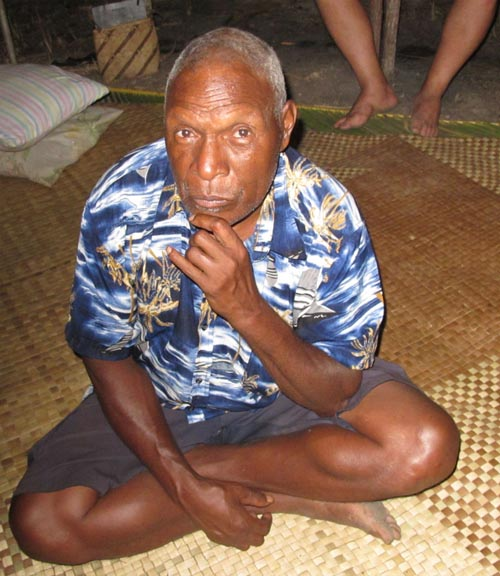
\includegraphics[width=.4\textwidth]{figures/foto-abia.jpg}
	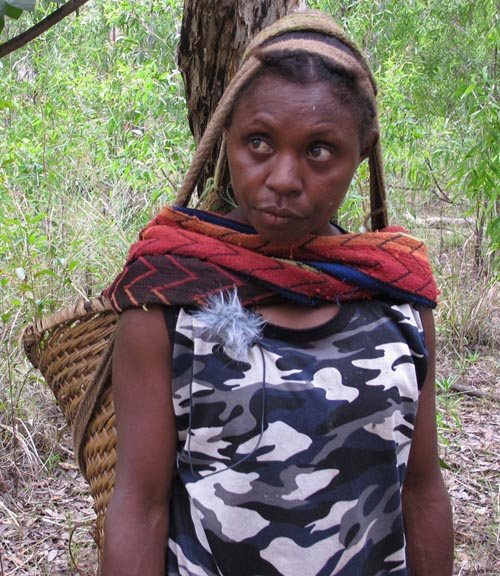
\includegraphics[width=.4\textwidth]{figures/foto-nakre.jpg}
  \caption{Abia and Nakre}
  \label{fig:abia-nakre}
\end{figure}

From 2011 onwards, the documentation of Komnzo was funded and supported by the \textsc{dobes} project of the Volkswagen Foundation.\footnote{\textsc{dobes} stands for \ili{German} `Dokumentation bedrohter Sprachen'.} The funding covered the basic documentation of two languages, namely Komnzo and \ili{Nen}, the language of Bimadbn village, on which Nick Evans has been working since 2008. The funding allowed us to buy a solar setup and ship it to both villages providing electricity for a computer, recording equipment and lights during the evening hours. Additionally, the \textsc{dobes} project supported to bring in academics who work in the field of biology. Kipiro Damas spent one week in Rouku in 2011 and again in 2015. He collected and later identified numerous plant specimens. Chris Healey identified and photographed over 100 bird species, thereby eliciting many fascinating narratives about cultural significance of birds. Julia Colleen Miller visited Rouku on two fieldtrips conducting socio-linguistic interviews as well as creating high-quality recordings suited for phonetic analysis.

\subsection{The text corpus}\label{thetextcorpus}

The last decade has seen an exceptional increase in creating and archiving digital language material. Despite this positive development, linguists have pointed out that this is ``unlikely to be parallelled by a significant acceleration in how long it takes field linguists to produce the sorts of careful translations and cross-questioning of semantic issues that are the hallmark of a well curated text collection'' (\citealt[25]{Evans:2006uu}). The authors employ the metaphor of a Russian Matryoshka doll to propose a structure of several subcorpora nested within each other, each one with increasing depth of analysis. The Komnzo \isi{corpus} follows this proposal. In fact, what I call the Komnzo \isi{corpus} here is only one-sixth of the material collected and archived within the project. At present, the \isi{archive} contains around 60 hours of audio-visual material. I estimate the total amount of text at around 40 hours.\footnote{This applies a wide notion of what consitutes a text, for example songs or wordlists would be included.} The material that has been segmented, transcribed and translated amounts to 12 hours, and this is the Komnzo text \isi{corpus}. These 12 hours constitute the data on which the description and analysis in this grammar rests. Hence, although around 60 hours have been archived, only 12 hours can be used for linguistic analysis. I hope that future speakers of Komnzo as well as researchers will benefit from the raw material.\\

The 12-hour \isi{corpus} contains narratives, procedurals, conversations, public speeches, interviews as well as recordings from various stimulus tasks. Most recording sessions took place in somewhat articifical settings, whether it be a staged narration or a sociolinguistic interview. All conversational texts and public speeches are purely observational. At the present time, the Komnzo \isi{corpus} consists of 65 texts with a total of 11hrs and 42min of transcribed material, and around 54,000 words. 34 speakers are featured in the age range from 20 to 68. The representation of speakers is skewed towards male speakers, 25 male versus 9 female. Furthermore, they are skewed towards speakers belonging to the Mayawa section. I acknowledge this as an artefact caused by the circumstances under which I was introduced to and later lived in Rouku.\\

The material has been placed in two locations. The complete material is archived at The Language Archive (TLA) which is a unit of the Max Planck Institute for Psycholinguistics, Nijmegen concerned with digital language resources and tools. The subset of files which make up the Komnzo text \isi{corpus} are also archived at Zenodo.\footnote{Zenodo is an open access repository for research related data which belongs to the European Council's OpenAIRE initiative.} At both locations, the materials are stored under an open-access policy. In order to access, browse and download the files, the reader can follow the links below:\\

\noindent
\fbox{\footnotesize{\href{https://archive.mpi.nl/islandora/object/lat\%3A1839\_00\_0000\_0000\_0017\_B0AC\_C}{https://archive.mpi.nl/islandora/object/lat\%3A1839\_00\_0000\_0000\_0017\_B0AC\_C}}}\\
\hfill\\
\fbox{\footnotesize{\href{https://zenodo.org/communities/komnzo}{https://zenodo.org/communities/komnzo}}}\\

There are over 500 examples in this grammar, and around 90\% of these are text examples. Text examples can be distinguished from elicited or overheard examples by an \isi{archive} ID printed in [angled brackets] underneath the example sentence. Elicited examples are not marked, while overheard examples are marked with [overheard]. The \isi{archive} ID allows the reader to find the example sentence in the text \isi{corpus} and thereby view the example in its context. Archive IDs follow a fixed structure. A example is: [tci20110810-02 MAB \#34]. The first three letters represent the ISO 639-3 code for Komnzo.\footnote{Note that Komnzo is listed, for example in Ethnologue, as a dialect of \ili{Wára}. Hence, the code `tci' includes more varieties than the one decribed in this grammar. More recent systems of language identification are more accurate in my opinion. For example, Glottolog lists Komnzo under the code: komn1238, which refers only to Komnzo.} The next eight digits and the number after the hyphen refer to the date on which the recording was made. For example, tci20110810-02 refers to the second recording session on the 10\super{th} of August 2011.  Hence, this information indentifies the particular transcription file within the \isi{corpus}. The last two elements of the \isi{archive} ID help to find a particular example in the transcription file. First, there is a three letter code which identifies the speaker, for example MAB for Marua Bai. If there are several speakers, each one is coded by a set of annotation tiers, all of which include the respective three letter code. The speaker code is followed by the annotation number, which refers to the sequence of intonation units on a tier.\\

This information is needed to find a particular line of text in the \isi{archive}. The reader of the electronic version of this grammar may simply click on the \isi{archive} ID, which is printed below each text example. This will take her directly to the list of recordings in the appendix. The list of recordings in the appendix provides general information about each text (title, text genre, length, number of annotation units, number of tokens) as well as about each speaker (name, age, sex, section/clan). Moreover, the list of recordings contains a digital object identifier (\textsc{doi}) that establishes a permanent link to the respective dataset on the Zenodo website. Practically, it should be no more than three mouseclicks to get from an example sentence to downloading the relevant transcription file. In this way, I enable the reader to access the original text without much effort.